\documentclass[12pt, a4paper]{article}
\usepackage{graphicx} % Required for inserting images
\usepackage[utf8]{vietnam}
\usepackage{amsmath,amsxtra,amssymb,latexsym,amscd,amsthm}
\usepackage[left=2cm,right=2cm,top=2cm,bottom=2cm]{geometry}
\usepackage{xcolor}
\usepackage{indentfirst}



\usepackage{enumitem,amssymb}
\newlist{todolist}{itemize}{2}
\setlist[todolist]{label=$\square$}
\usepackage{pifont}
\newcommand{\cmark}{\ding{51}}%
\newcommand{\xmark}{\ding{55}}%
\newcommand{\done}{\rlap{$\square$}{\raisebox{2pt}{\large\hspace{1pt}\cmark}}%
\hspace{-2.5pt}}
\newcommand{\wontfix}{\rlap{$\square$}{\large\hspace{1pt}\xmark}}


\usepackage{dirtree}
\usepackage{pythonhighlight}
\usepackage{minted}
\usepackage{fontawesome}

%%-------------------------------------------------------------


\begin{document}

%%-------------------------------------------------------------
\noindent
\begin{center}
\fontsize{15}{17}\selectfont
\color{black}\textbf{BỘ     GIÁO DỤC VÀ ĐÀO TẠO}\\
\color{blue}\textbf{TRƯỜNG ĐẠI HỌC SƯ PHẠM KỸ THUẬT TP.HCM}\\
\color{black}\textbf{KHOA CƠ KHÍ CHẾ TẠO MÁY}\\

\vspace{50px}
\begin{figure}[h]
    \centering
    
\includegraphics[scale=0.8]{Img/logo}
\end{figure}
\vspace{30px}

\fontsize{18}{15}\selectfont
\textbf{BÁO CÁO GIỮA KÌ}\\
\fontsize{24}{18}\selectfont
\color{red}\textbf{ TRÍ TUỆ NHÂN TẠO}\\
\fontsize{13}{13}
\textbf{NHẬN DIỆN HÌNH ẢNH BẰNG PHƯƠNG PHÁP DEEP LEARNING (Convolutional Neural Network - CNN)}


\vspace{50px}

\end{center}


\fontsize{12}{17}\selectfont
\setlength{\parindent}{0cm}
\color{black} \textbf{GIẢNG VIÊN HƯỚNG DẪN:}\hspace{1cm}\color{blue} \textbf{PGS.TS NGUYỄN TRƯỜNG THỊNH} 
\par \color{black} \textbf{Mã Học Phần: }\hspace{4.2cm}\color{blue}\textbf{222ARIN337629E}
\par \color{black} \textbf{HỌ $\&$ TÊN SINH VIÊN:}\hspace{2cm} \color{blue} \textbf{Nguyễn Ngọc Nhân} \\
\color{black} \textbf{MSSV:}\hspace{6cm}\color{blue} \textbf{20146262} \\

\vspace{80px}

\begin{center}
    

\fontsize{13}{17}\selectfont
\color{black}\textbf{TP Hồ Chí Minh, ngày 30 tháng 4 năm 2023}


\end{center}

%-------------------------------------------------------------
\color{black}


\newpage
\begin{center}
\tableofcontents
\end{center}

%-------------------------------------------------------------
\newpage
\section{Introduction - Giới thiệu}
\par \hspace{1cm}- Convolutional Neural Network (CNN – Mạng nơ-ron tích chập) là một trong những mô hình Deep Learning (DL) tiên tiến để nhận dạng và phân loại hình ảnh. Nó giúp cho chúng ta xây dựng được những hệ thống thông minh với độ chính xác cao như hiện nay.
\par \hspace{1cm}- CNN được áp dụng rộng rãi trong nhiều lĩnh vực hiện nay, bao gồm việc nhận diện khuôn mặt, phân loại bênh qua ảnh chụp từ y khoa, phát hiện các object (vật thể) qua các video và hình ảnh. Với sự phát triển liên tục, CNN đã đóng vai trò quan trọng trong việc giải quyết các vấn đề về lĩnh vực thị giác máy tính.
%-------------------------------------------------------------
\section{Methodology - Phương pháp}
\begin{figure}[h] %% [h] --> here
    \centering
    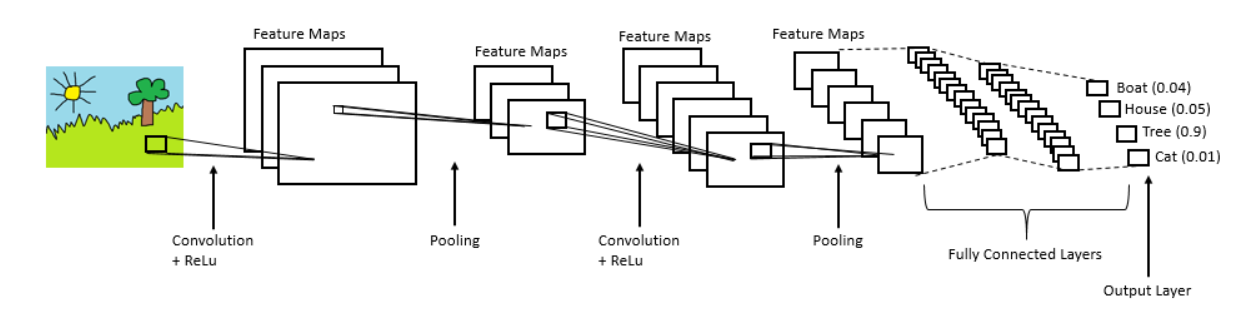
\includegraphics[scale = 0.67]{Img/cnn2.png}
\end{figure}


\subsection{Convolution Layer - Lớp tính chập}
\par \hspace{1cm}- Là lớp đầu tiên để trích xuất các tính năng từ hình ảnh đầu vào. Nó sử dụng phép tính  toán convolution (tích chập) giữa các ma trận. Tức là, nó áp dụng một kernel (còn được gọi là filter hoặc weight) đến một vùng của ảnh đầu vào để tạo ra một feature map (bản đồ đặc trưng) mới. 
\par \hspace{1cm}- Việc tính toán này được thực hiện bằng cách áp dụng phép nhân ma trận giữa kernel và các phần tử tương ứng trên vùng ảnh đầu vào, sau đó tính tổng các kết quả và lưu vào feature map. Quá trình này được thực hiện trên toàn bộ ảnh đầu vào để tạo ra nhiều feature map khác nhau, từ đó trích xuất các đặc trưng của ảnh để phục vụ cho các mục đích như phân loại, nhận dạng, phát hiện.
\begin{figure}[h] %% [h] --> here
    \centering
    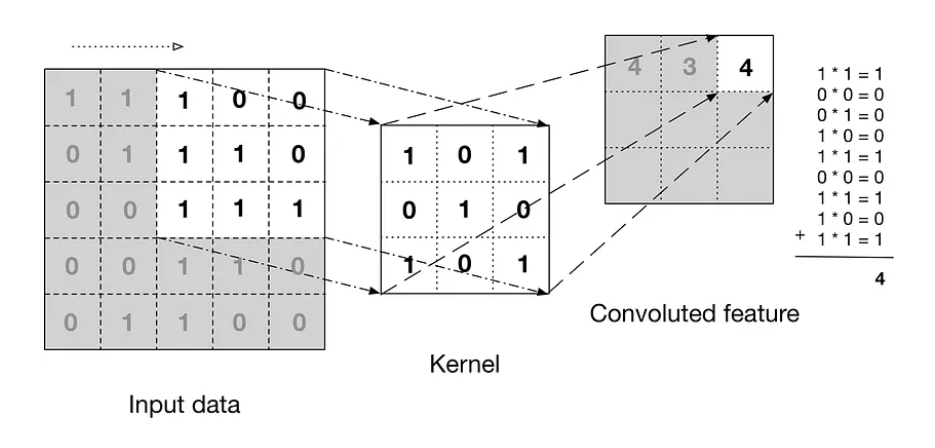
\includegraphics[scale = 0.6]{Img/ConvL2.png}
\end{figure}

\par \hspace{1cm}- Sự kết hợp của 1 hình ảnh với các bộ lọc khác nhau có thể giúp chúng ta tìm ra cạnh, làm mờ và làm sắc nét bằng cách áp dụng các bộ lọc. 
\par \hspace{1cm}- Ví dụ dưới đây cho thấy hình ảnh tích chập khác nhau sau khi áp dụng các Kernel khác nhau.
\begin{figure}[h] %% [h] --> here
    \centering
    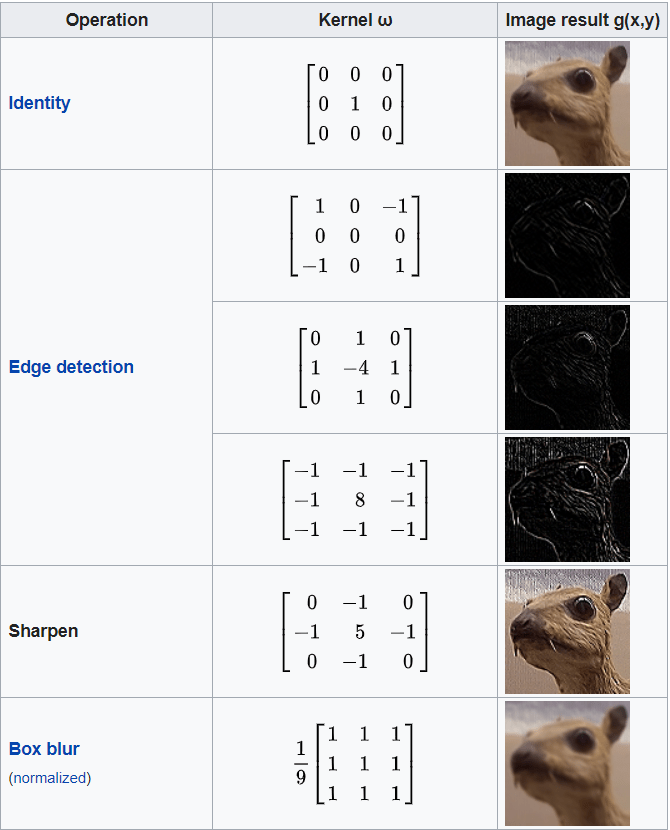
\includegraphics[scale = 0.45]{Img/cvl.png}
\end{figure}


\subsection{Stride - Bước nhảy}
\par \hspace{1cm}-  Stride giúp ta xác định bao nhiêu pixel bước đi mỗi lần trượt bộ lọc tích chập trên ma trận đầu vào. 
\par \hspace{1cm}- Ví dụ khi stride là 1 tức là di chuyển các kernel 1 pixel. Khi stride là 2 tức là di chuyển các kernel đi 2 pixel và tiếp tục như vậy.
\par \hspace{1cm}- Ví dụ hình ảnh dưới đây mô tả lớp chập hoạt động với stride là 2.
\begin{figure}[h] %% [h] --> here
    \centering
    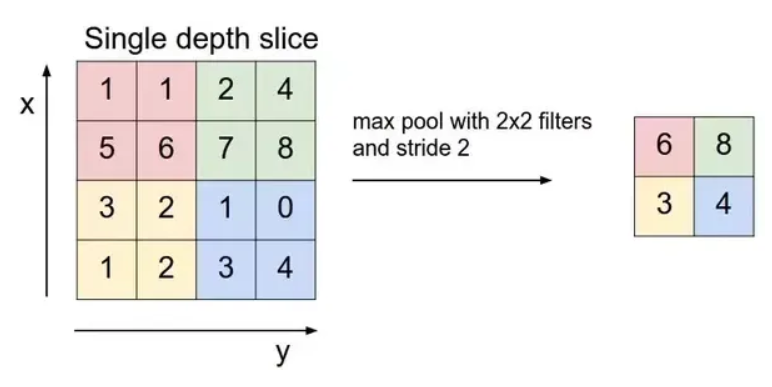
\includegraphics[scale = 0.52]{Img/stride1.png}
\end{figure}

\newpage
\subsection{Padding - Đường viềng}
\par \hspace{1cm}- Để giải quyết một số trường hợp kernel không phù hợp với ảnh đầu vào vì sau mỗi lần thực hiện phép tính convolution xong thì kích thước ma trận output - Y đều nhỏ hơn ma trận input - X. Ta chọn tăng kích thước ảnh bằng cách thêm padding. Tức là thêm giá trị 0 ở viền ngoài ma trận X.
\par \hspace{1cm}- Ví dụ dưới đây là thêm giá trị 0 ở viền với paddding = 1.
\begin{figure}[h] %% [h] --> here
    \centering
    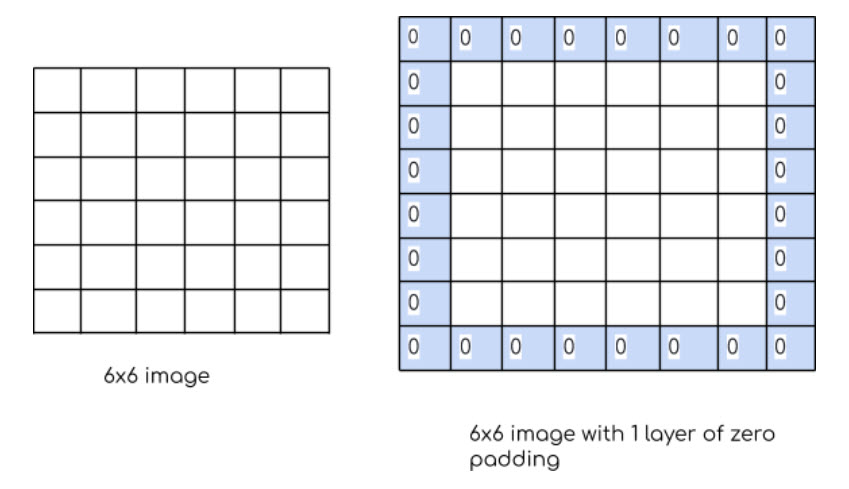
\includegraphics[scale = 0.8]{Img/padding1.jpg}
\end{figure}

\par \hspace{1cm}- Phép tính này được gọi là convolution với padding=1. Khi padding = k nghĩa là ta thêm k vector 0 vào mỗi phía của ma trận.


\subsection{Rectified Linear Unit (Relu) - Hàm phi tuyến}
\par \hspace{1cm}- Giúp mạng neural học các đặc trưng tốt hơn và tăng tốc quá trình hội tụ trong quá trình huấn luyện.
\par \hspace{1cm}- Giảm thiểu hiện tượng Gradient Vanishing (tức là khi gradient giảm đáng kể đến mức rất gần bằng 0 làm các trọng số của mạng neuron được cập nhật rất chậm hoặc thậm chí không cập nhật được nữa). 
\par \hspace{1cm}- Đầu ra $f(x) = max(0, x)$ . Tức là ma trận sau khi thực hiện phép tính chập và áp dụng hàm Relu ta sẽ ra được một ma trận không âm
\begin{figure}[h] %% [h] --> here
    \centering
    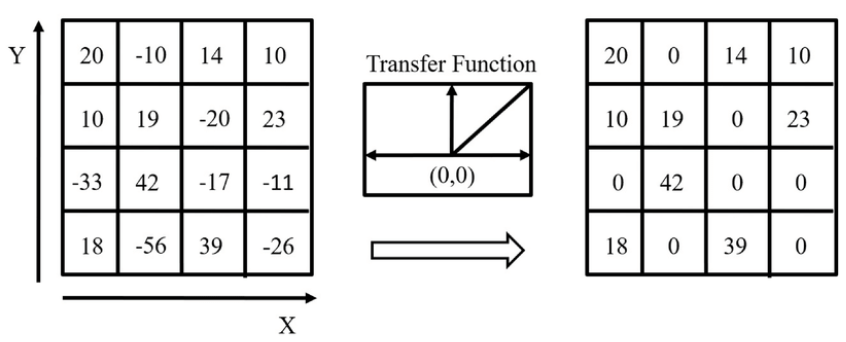
\includegraphics[scale = 0.6]{Img/Relu1.png}
\end{figure}
\par \hspace{1cm}- Tuy nhiên các node có giá trị nhỏ hơn 0, qua ReLU activation sẽ thành 0, hiện tượng này gọi là “Dying ReLU“. Khi các node bị chuyển thành 0 sẽ không còn ý nghĩa với linear activation ở lớp tiếp theo và các hệ số tương ứng từ node đấy cũng không được cập nhật với gradient descent (vì bằng 0 nên không thể gradient được). $\Rightarrow$ Leaky ReLU ra đời.

\newpage
\subsection{Pooling Layer - Lớp gộp}
\par \hspace{1cm}- Để giảm bớt kích thước đầu vào và trích xuất các đặc trưng quan trọng.
\par \hspace{1cm}- Thường được dùng giữa các convolutional layer.
\par \hspace{1cm}- Có 2 loại pooling layer phổ biến là max pooling và average pooling:
\par \hspace{2cm}+ Max pooling là pooling layer sẽ chọn ra giá trị lớn nhất trong mỗi khối \par \hspace{2.4cm}đó để đưa ra đầu ra.
\par \hspace{2cm}+ Average pooling là pooling layer sẽ lấy giá trị trung bình trong mỗi khối
\par \hspace{2.4cm}để đưa ra đầu ra.


\begin{figure}[h] %% [h] --> here
    \centering
    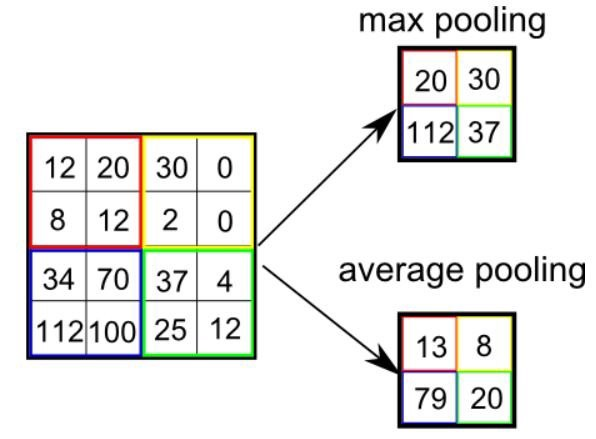
\includegraphics[scale = 0.4]{Img/pool.png}
\end{figure}


\subsection{Forward Pass and Backward Pass - chạy thuận và chạy nghịch}
\par \hspace{1cm}- Forward Pass là quá trình đưa dữ liệu đầu vào đi qua một mạng neural network, các phép tính được thực hiện từ lớp đầu vào đến lớp đầu ra và cho ra kết quả đầu ra.
\par \hspace{1cm}- Backward pass là quá trình tính toán đạo hàm (gradient) của hàm mất mát theo các tham số của mạng neural network. Quá trình này được thực hiện bằng thuật toán backpropagation, từ lớp đầu ra trở về lớp đầu vào, giúp cho việc cập nhật các trọng số mạng để tối ưu hoá mô hình được thực hiện một cách hiệu quả.
\begin{figure}[h] %% [h] --> here
    \centering
    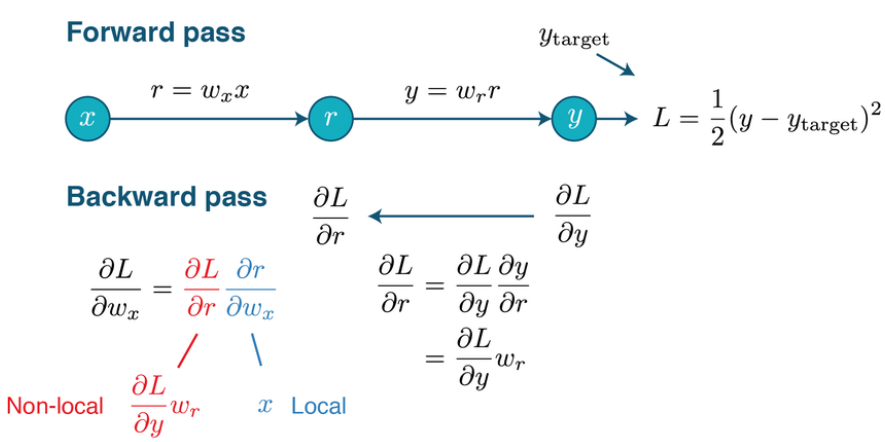
\includegraphics[scale = 0.8]{Img/ForBack.png}
\end{figure}

%-------------------------------------------------------------
\newpage
\section{Implementation - Thực hiện}


\par \textbf{Các bước thực hiện}
\par\hspace{0.5cm}+ \textbf{Step 1}: Thu thập dữ liệu
\par\hspace{0.5cm}+ \textbf{Step 2}: Xử lý dữ liệu
\par\hspace{0.5cm}+ \textbf{Step 3}: Xây dựng model CNN
\par\hspace{0.5cm}+ \textbf{Step 4}: Viết hàm loss đánh giá
\par\hspace{0.5cm}+ \textbf{Step 5}: Nhập ảnh đầu vào từ tập test và demmo kết quả

\vspace{0.5cm}
\par\textbf{Công việc đã thực hiện} 

\begin{itemize}
    \item
    \begin{todolist}
        
        \item[\done]Xây dựng model CNN với frame-work.
        
        \begin{todolist}
        \item[\done] Pytorch
        \item Keras %[\wontfix]
        \item TensorFlow
        \end{todolist}
        
    \end{todolist}
    
    \item 
    \begin{todolist}
        \item[\done] Demo kết quả.
        \begin{todolist}
        \item[\done] Demo kết quả trên ảnh
        \item Demo kết quả trên video
        \end{todolist}
        
    \end{todolist}

    \item 
    \begin{todolist}
        \item[\done] Trực quan hóa và theo dõi các chỉ số quá trình huấn luyện.
        \begin{todolist}
        \item[\done] TensorBoard
        \end{todolist}
        
    \end{todolist}
    
\end{itemize}



\vspace{0.5cm}

\par \textbf{Cấu trúc dataset chung.} 
\dirtree{%
.1 Dataset.
.2 Train.
.3 Label-1.
.4 img-1.jpg.
.4 img-2.jpg.
.4 ....
.4 img-n.jpg.
.3 Label-2.
.3 ....
.3 Label-n.
.2 Valid.
.3 Label-1.
.4 img-1.jpg.
.4 img-2.jpg.
.4 ....
.4 img-n.jpg.
.3 Label-2.
.3 ....
.3 Label-n.
.2 Test.
.3 Label-1.jpg.
.3 Label-2.jpg.
.3 ....
.3 Label-n.jpg.
}
 








\newpage
\subsection{Prediction of your future based on hand palm outline or face or fingerprint.  }
\par \textbf{Code đầy đủ ở đây [6]}
\par\hspace{0cm}- Đầu tiên ta sẽ import các thư viện cần thiết cho việc xây dựng và thực thi model
\par\hspace{0cm}- Ở đây ta sẽ dùng Cuda cho việc xây model trên GPU và nó giúp ta tăng tống quá trình train và thực thi model
\begin{python}
In [1]: import numpy as np
        from tqdm import tqdm
        import torch
        import torch.nn as nn
        import torchvision
        import torch.nn.functional as F
        from torch.utils.data import DataLoader
        from torchvision import datasets, transforms, models
        from torchvision.transforms import ToTensor
        import matplotlib.pyplot as plt
        from torch.utils.tensorboard import SummaryWriter
        
        
        device = torch.device('cuda' if torch.cuda.is_available() else 'cpu')
        print(device)
\end{python}
\begin{minted}{bash}
Out [1]: cuda

\end{minted}

\par - Tiếp Theo ta sẽ xây dựng hàm \textbf{transform}  để biến đổi trên dữ liệu (data augmentation) hoặc chuẩn hóa (data normalization) dữ liệu trước khi đưa vào huấn luyện mô hình.
\par - Việc sử dụng hàm \textbf{transform} giúp cho mô hình huấn luyện được đào tạo trên nhiều dữ liệu đa dạng hơn, giúp mô hình học được các đặc trưng tổng quát hơn và tránh overfitting trên dữ liệu huấn luyện.
\par - Quy trình của hàm \textbf{transform}: Thay đổi kích thước ảnh về dạng (124x124) $\Rightarrow$ đưa ảnh về dạng các cạnh dựa vào hàm \textbf{Canny()} $\Rightarrow$ Đưa ma trận ảnh về dạng \textbf{tensor} để làm việc  với pytorch.
\begin{python}
In [2]: from PIL import Image
        import torch
        from torchvision import transforms
        import cv2
        
        class CannyEdgeTransform:
            def __init__(self, threshold1=100, threshold2=220):
                self.threshold1 = threshold1
                self.threshold2 = threshold2
                
            def __call__(self, img):
                # Chuyen PIL.Image sang numpy array
                img_np = np.array(img)
                # Chuyen sang anh grayscale
                img_gray = cv2.cvtColor(img_np, cv2.COLOR_BGR2GRAY)
                # Ap dung edge detection bang Canny
                edges = cv2.Canny(img_gray, self.threshold1, self.threshold2)
                
                # Chuyen lai PIL.Image
                edges_pil = Image.fromarray(edges)
                # Ap dung transform cua Pytorch
                edges_tensor = transforms.ToTensor()(edges_pil)
                return edges_tensor
            
            
        transform = transforms.Compose([
            transforms.Resize(124), # thay doi kich thuoc ben ngan nhat thanh 124 pixel             
            transforms.CenterCrop(124), # cat kich thuoc ben dai nhat ra khoang 124 pixel tu trung tam 
            CannyEdgeTransform(threshold1=100, threshold2=220) # chuyen anh ve dang canny edge de thay duoc net mat nguoi
        ])
        x_train = FaceDataset(root=("/kaggle/input/face-class/Face/Train"), transform = transform)
        x_val = FaceDataset(root = ('/kaggle/input/face-class/Face/Val'), transform = transform)
\end{python}

- Đầu vào là hình ảnh mặt người sau đó ta sẽ xác định và cắt vùng ảnh chứa mặt người về kích thước (124x124) sau đó ta sẽ dùng hàm \textbf{CannyEddgeTransform()} dể chuyển về dạng các cạnh.


\begin{python}
In [3]: import matplotlib.pyplot as plt
        
        # Load anh goc
        img = Image.open('/kaggle/input/face-class/Face/Train/NguyenNgocNhan/img1.jpg')
        
        # Hien thi anh goc
        plt.subplot(1, 2, 1) # 1 hang, 2 cot, vi tri 1
        plt.imshow(img)
        
        # Chuyen tensor ve numpy array va doi lai thu tu cac kenh mau
        transformed_img = transform(img).numpy().transpose(1, 2, 0) 
        # Tensor: (C, H, W) -> OpenCV, Matlab: (H, W, C)
        
        # Hien thi anh sau khi ap dung transform
        plt.subplot(1, 2, 2) # 1 hang, 2 cot, vi tri 2
        plt.imshow(transformed_img, cmap='gray')
        
        # Hien thi dong thoi
        plt.show()
\end{python}
\newpage
\begin{minted}{bash}
Out [3]: 
\end{minted}
\begin{figure}[h] %% [h] --> here
    \centering
    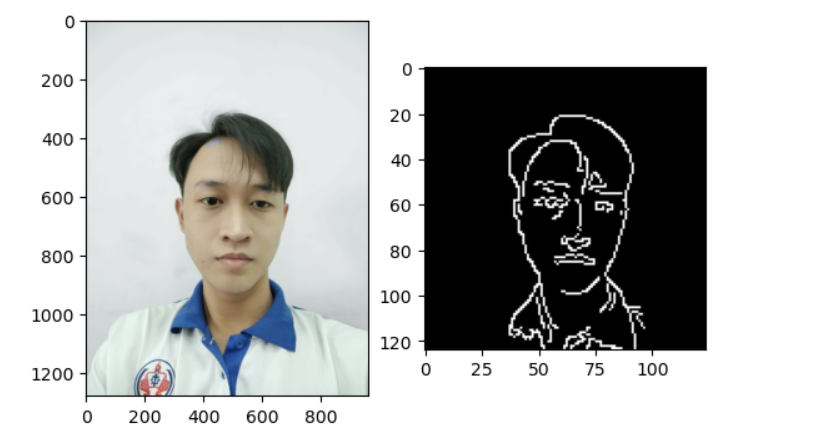
\includegraphics[scale = 0.8]{Img/Pre_Fut/P1.png}
\end{figure}

\begin{python}
In [4]: print("Tong class: ",len(x_train.classes))
        class_predict_future = ['Ca si', 'Game thu', 'Trader', 'Ky su PID', 'Ky su']
        print("Cac du doan co the: ",class_predict_future)
\end{python}
\begin{minted}{bash}
Out [4]: Tong class:  5
         Cac du doan co the:  ['Ca si', 'Game thu', 'Trader', 'Ky su PID', 'Ky su'] 

\end{minted}

\par - Tiếp theo ta  sẽ tiến hành thiết lập siêu tham số (hyperparameter) và chia dữ liệu theo batch cho model
\par - Ở đây ta sử dụng Weight Decay (L2 Regularization) bằng 0.0001 để giảm thiểu Overfitting [5]
\begin{python}
In [5]: batch = 128 # Khai bao kich thuoc batch
        epochs = 12 # Thuc hien 80 epochs
        learning_rate = 1e-3 # Khao bao toc do hoc la 10^(-3)
        weight_decay = 1e-4 # Khai bao weight decay la 10^(-4) de giam thieu overfitting
        
        train_loader = DataLoader(x_train, batch_size = batch, shuffle = True)
        val_loader = DataLoader(x_val, batch_size = batch, shuffle = True)
\end{python}
\par - Tiếp theo ta sẽ tiến hành xây dựng model CNN
\par - Dưới đây là hình ảnh cấu trúc model CNN. Chi tiết xem thêm tại đây[11]
\newpage
\begin{figure}[h] %% [h] --> here
    \centering
    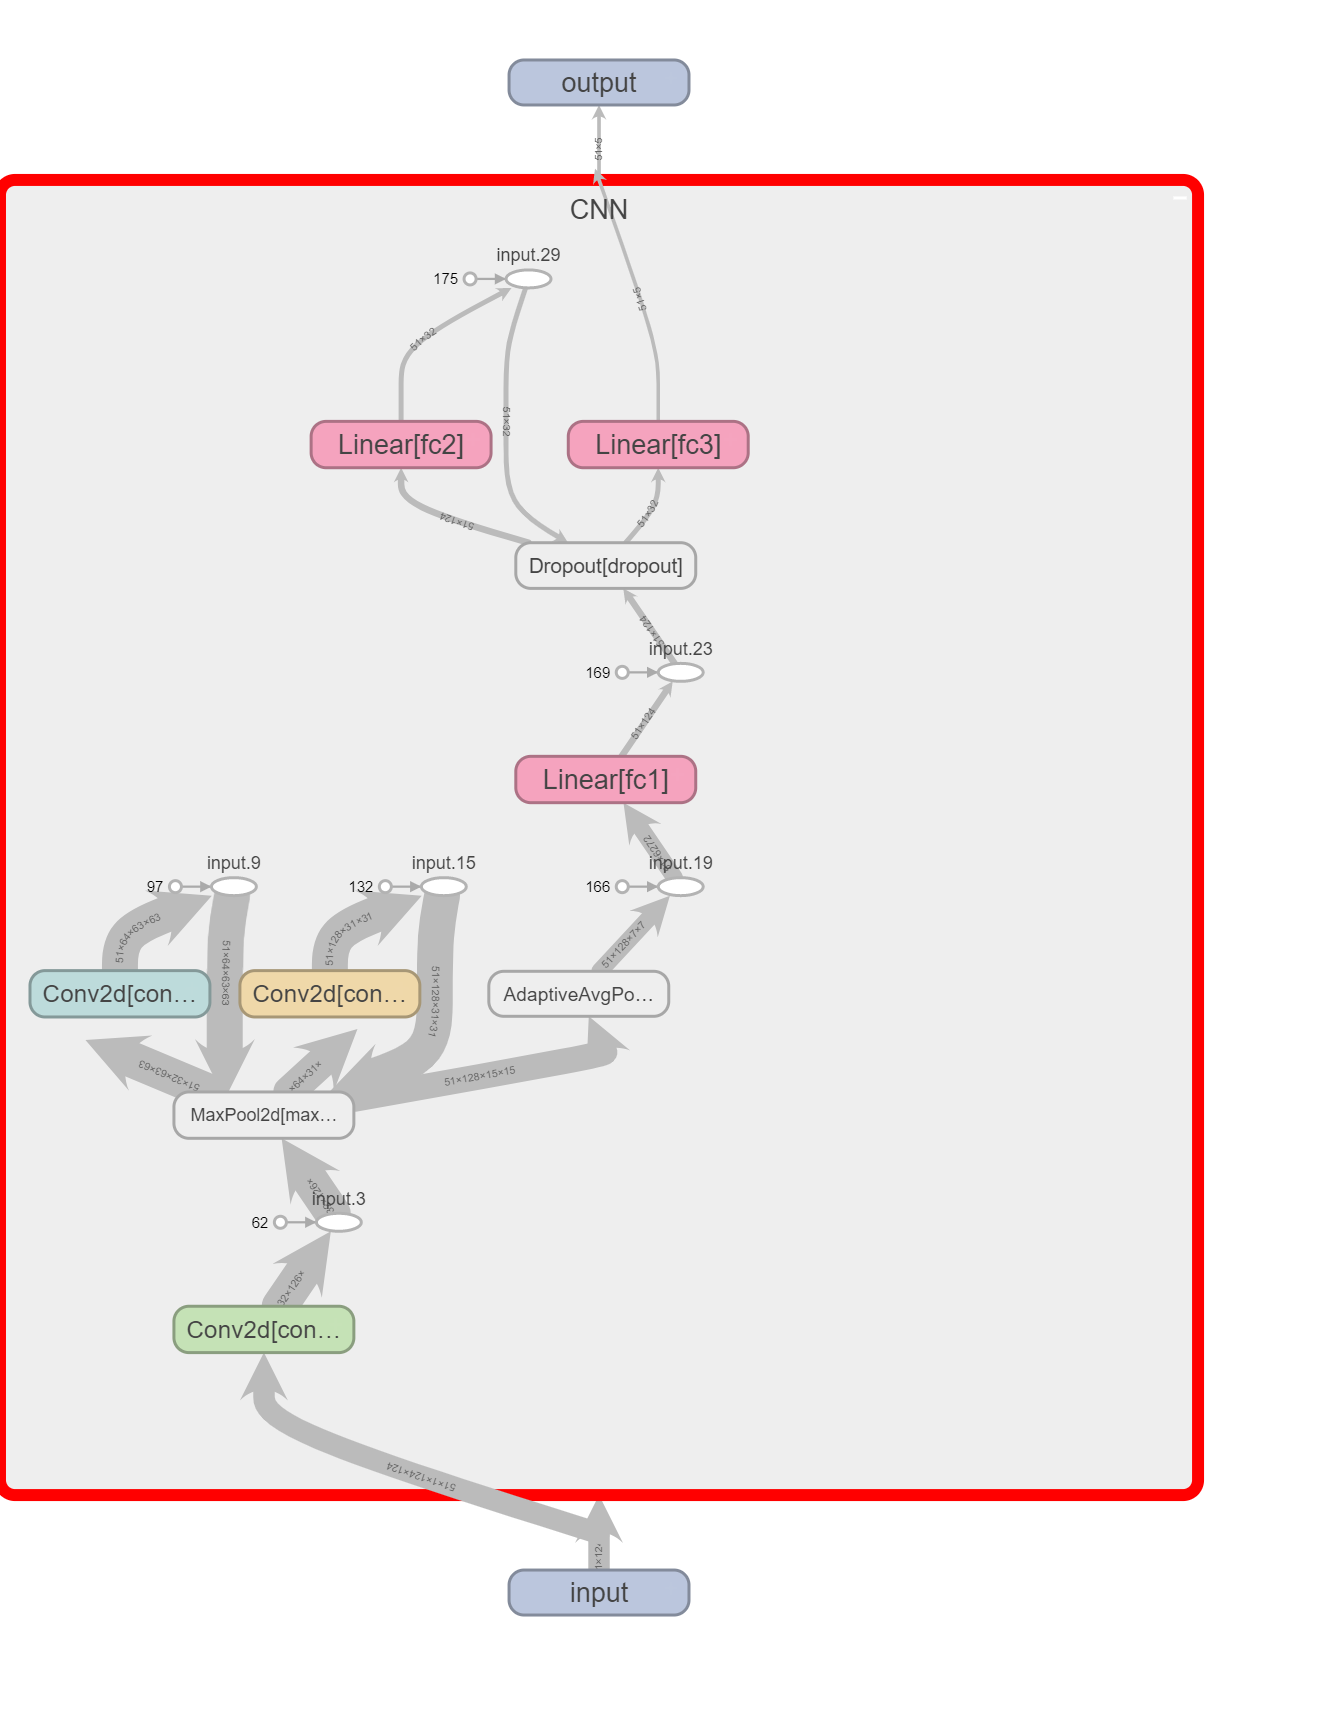
\includegraphics[scale = 0.2]{Img/Pre_Fut/P4.png}
\end{figure}
\begin{python}
In [6]:class CNN(nn.Module):
          def __init__(self):
            super(CNN, self).__init__()
            self.maxpool = nn.MaxPool2d(kernel_size = 2, stride = 2)
            self.conv1 = nn.Conv2d(1,32,3,stride = 1, padding = 2)
            self.conv2 = nn.Conv2d(32,64,3,stride = 1, padding = 1)
            self.conv3 = nn.Conv2d(64,128,3,stride = 1, padding = 1)
            self.avgpool = nn.AdaptiveAvgPool2d((7, 7))
            self.dropout = nn.Dropout(p = 0.1)
            self.fc1 = nn.Linear(7*7*128, 124)
            self.fc2 = nn.Linear(124,32)
            self.fc3 = nn.Linear(32, 5)

            
          def forward(self, x):
            x = self.maxpool(F.leaky_relu(self.conv1(x)))
            x = self.maxpool(F.leaky_relu(self.conv2(x)))
            x = self.maxpool(F.leaky_relu(self.conv3(x)))
            x = self.avgpool(x)
            x = x.view(-1, 7*7*128)
            x = self.dropout(F.leaky_relu(self.fc1(x)))
            x = self.dropout(F.leaky_relu(self.fc2(x)))
            x = self.fc3(x)
        
            return x
        
        model = CNN().to(device)
        criterion = nn.CrossEntropyLoss()
        optimizer = torch.optim.Adam(model.parameters(), lr = learning_rate, weight_decay = weight_decay)
\end{python}

\begin{python}
In [7]: from prettytable import PrettyTable
        
        def count_parameters(model):
            table = PrettyTable(["Modules", "Parameters"])
            total_params = 0
            for name, parameter in model.named_parameters():
                if not parameter.requires_grad: 
                    continue
                param = parameter.numel()
                table.add_row([name, param])
                total_params+=param
            print(table)
            print(f"Total Trainable Params: {total_params}")
            return total_params
        
        count_parameters(model)
\end{python}
\begin{minted}{bash}
        +--------------+------------+
        |   Modules    | Parameters |
        +--------------+------------+
        | conv1.weight |    288     |
        |  conv1.bias  |     32     |
        | conv2.weight |   18432    |
        |  conv2.bias  |     64     |
        | conv3.weight |   73728    |
        |  conv3.bias  |    128     |
        |  fc1.weight  |   777728   |
        |   fc1.bias   |    124     |
        |  fc2.weight  |    3968    |
        |   fc2.bias   |     32     |
        |  fc3.weight  |    160     |
        |   fc3.bias   |     5      |
        +--------------+------------+
        Total Trainable Params: 874689

Out [7]: 874689

\end{minted}
\par - Tổng có 874689 tham số
\vspace{0.5cm}
\newpage
\par - Tiếp theo ta sẽ tiến hành train và đánh giá model
\begin{python}
In [8]:

n_total_steps = len(train_loader)
run_loss = 0.0
run_acc = 0.0
for epoch in range(epochs):
    for i, (images, labels) in enumerate(tqdm(train_loader)):
        images = images.reshape(-1,1,124,124).to(device)
        labels = labels.to(device)
        _, labels = torch.max(labels.data, 1)
        outputs = model(images)
        loss = criterion(outputs,labels)
        run_loss +=loss.item() #for tensorboard
        _,pred = torch.max(outputs.data, 1)
        run_acc += (pred==labels).sum().item()#for tensorboard
        
        optimizer.zero_grad()
        loss.backward()
        optimizer.step()
        
        if (i+1) % 2 == 0:
            with torch.no_grad():
                n_correct = 0
                n_samples = 0
                n_class_correct = [0 for i in range(5)]
                n_class_samples = [0 for i in range(5)]
                
                for images_val, labels_val in val_loader:
                    images_val = images_val.reshape(-1,1,124,124).to(device)
                    labels_val = labels_val.to(device)
                    _, labels_val = torch.max(labels_val.data, 1)
                    output_val = model(images_val)
                    _, predict_val = torch.max(output_val.data, 1)
                    n_samples += labels_val.size(0)
                    n_correct += (predict_val == labels_val).sum().item()
                    loss_val = F.mse_loss(labels_val.float(),predict_val.float())
                    for i in range(26):
                        label_val = labels_val[i]
                        pred_val = predict_val[i]
                        if label_val == pred_val:
                            n_class_correct[label_val] += 1
                        n_class_samples[label_val] += 1
                        
                acc_val = n_correct/(n_samples)  
                run_acc_result = run_acc/((2-1)*128+pred.size(0))
                print(f'Epoch[{epoch+1}/{epochs}]:  Loss_Train: {(run_loss/2):.2f}, Acc_Train: {run_acc_result:.2f} , Loss_Val: {loss_val:.2f} , Acc_Val: {acc_val:.2f} ')
            
            run_loss = 0.0
            run_acc = 0.0

print('Finished Training')
\end{python}
\newpage
\begin{minted}{bash}
Out [8]:
100%[==========] 2/2 [00:15<00:00,  7.99s/it]
Epoch[1/12]: Loss_Train: 1.60, Acc_Train: 0.17, Loss_Val: 4.41, Acc_Val: 0.14 
100%[==========] 2/2 [00:15<00:00,  7.77s/it]
Epoch[2/12]: Loss_Train: 1.56, Acc_Train: 0.36, Loss_Val: 2.41, Acc_Val: 0.29 
100%[==========] 2/2 [00:15<00:00,  7.96s/it]
Epoch[3/12]: Loss_Train: 1.44, Acc_Train: 0.30, Loss_Val: 2.49, Acc_Val: 0.45 
100%[==========] 2/2 [00:15<00:00,  7.68s/it]
Epoch[4/12]: Loss_Train: 1.19, Acc_Train: 0.62, Loss_Val: 1.12, Acc_Val: 0.76 
100%[==========] 2/2 [00:15<00:00,  7.93s/it]
Epoch[5/12]: Loss_Train: 0.89, Acc_Train: 0.75, Loss_Val: 1.29, Acc_Val: 0.75 
100%[==========] 2/2 [00:15<00:00,  7.73s/it]
Epoch[6/12]: Loss_Train: 0.54, Acc_Train: 0.78, Loss_Val: 1.35, Acc_Val: 0.80 
100%[==========] 2/2 [00:16<00:00,  8.11s/it]
Epoch[7/12]: Loss_Train: 0.38, Acc_Train: 0.90, Loss_Val: 0.22, Acc_Val: 0.90 
100%[==========] 2/2 [00:15<00:00,  7.68s/it]
Epoch[8/12]: Loss_Train: 0.32, Acc_Train: 0.90, Loss_Val: 0.53, Acc_Val: 0.90 
100%[==========] 2/2 [00:16<00:00,  8.09s/it]
Epoch[9/12]: Loss_Train: 0.11, Acc_Train: 0.97, Loss_Val: 0.35, Acc_Val: 0.92 
100%[==========] 2/2 [00:15<00:00,  7.69s/it]
Epoch[10/12]: Loss_Train: 0.20, Acc_Train: 0.94, Loss_Val: 0.16, Acc_Val: 0.96 
100%[==========] 2/2 [00:16<00:00,  8.03s/it]
Epoch[11/12]: Loss_Train: 0.21, Acc_Train: 0.94, Loss_Val: 0.25, Acc_Val: 0.96 
100%[==========] 2/2 [00:15<00:00,  7.70s/it]
Epoch[12/12]: Loss_Train: 0.10, Acc_Train: 0.99, Loss_Val: 0.25, Acc_Val: 0.96 
Finished Training
\end{minted}
\begin{python}
In [9]: with torch.no_grad():
            n_correct = 0
            n_samples = 0
            n_class_correct = [0 for i in range(5)]
            n_class_samples = [0 for i in range(5)]
            for images, labels in val_loader:
                images = images.reshape(-1,1,124,124).to(device)
                labels = labels.to(device)
                _, labels = torch.max(labels.data, 1)
                output = model(images)
                _, predict = torch.max(output.data, 1)
                n_samples += labels.size(0)
                n_correct += (predict == labels).sum().item()
                for i in range(51):
                    label = labels[i]
                    pred = predict[i]
                    if label == pred:
                        n_class_correct[label] +=1
                    n_class_samples[label]+=1
            acc = 100.0*n_correct/n_samples
            print(f'Accuracy of the network: {acc} %')
\end{python}

\begin{minted}{bash}
Out [9]: Accuracy of the network: 96.07843137254902 %   
\end{minted}
\par - Sau 12 epochs ta có thể thấy độ chính xác trên tập validation là 96$\%$
\par - Dưới dây là dồ thị của độ chính xác. Màu tím của tập train và màu cam của tập validation. Chi tiết xem thêm tại đây [11]
\begin{figure}[h] %% [h] --> here
    \centering
    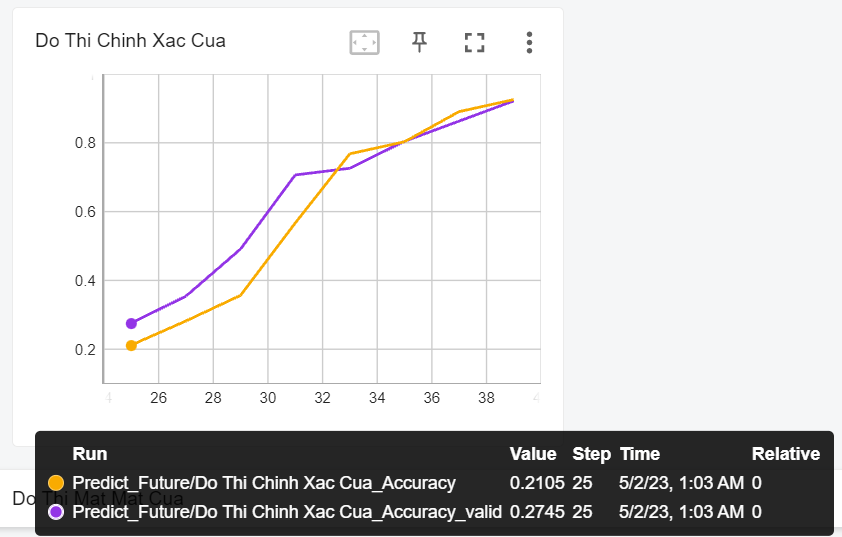
\includegraphics[scale = 0.6]{Img/Pre_Fut/P5.png}
\end{figure}

\par - Dưới dây là dồ thị của độ mất mát. Màu xanh của tập train và màu hồng của tập validation. Chi tiết xem thêm tại đây [11]
\begin{figure}[h] %% [h] --> here
    \centering
    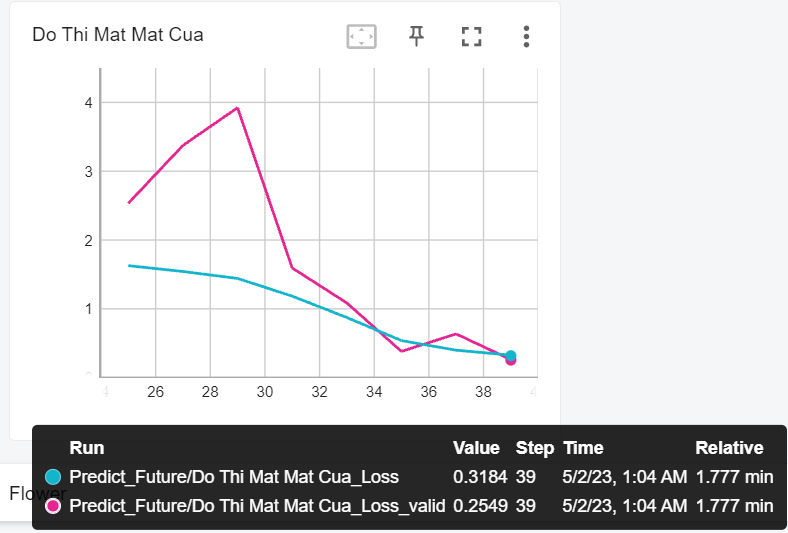
\includegraphics[scale = 0.65]{Img/Pre_Fut/P6.png}
\end{figure}
\newpage
\par - Tiến hành lưu và load model 

\begin{python}
In [10]:# Save model
        FILE = "model_face.pth"
        torch.save(model.state_dict(), FILE)
        # Load model
        loaded_model = CNN().to(device)
        loaded_model.load_state_dict(torch.load(FILE)) 
        loaded_model.eval()
\end{python}

\begin{minted}{bash}
Out [10]:
    CNN(
      (maxpool): MaxPool2d(kernel_size=2, stride=2, padding=0, dilation=1,
                            ceil_mode=False)
      (conv1): Conv2d(3, 32, kernel_size=(3, 3), stride=(1, 1), padding=(2, 2))
      (conv2): Conv2d(32, 64, kernel_size=(3, 3), stride=(1, 1), padding=(1, 1))
      (conv3): Conv2d(64, 128, kernel_size=(3, 3), stride=(1, 1), padding=(1, 1))
      (avgpool): AdaptiveAvgPool2d(output_size=(7, 7))
      (dropout): Dropout(p=0.1, inplace=False)
      (fc1): Linear(in_features=6272, out_features=124, bias=True)
      (fc2): Linear(in_features=124, out_features=32, bias=True)
      (fc3): Linear(in_features=32, out_features=6, bias=True)
    )
    
\end{minted}

\begin{python}
In [11]: # Tien hanh du doan tuong lai voi input la anh mat nguoi
        from torchvision import transforms
        import PIL.Image as Image
        url = '/kaggle/input/face-class/Face/Test/Trader.jpg'
        # Load anh
        img = Image.open(url)
        # Hien thi anh
        plt.imshow(img)
        plt.show()
        # Ap dung transform
        img_transformed = transform(img)
        # App load model
        test = loaded_model(img_transformed.to(device))
        print("Tuong lai lam: ",class_predict_future[torch.max(test.data,1)[1].data])
\end{python}


\begin{figure}[h] %% [h] --> here
    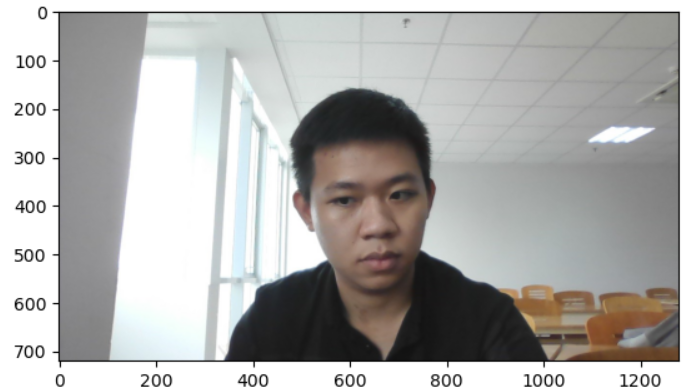
\includegraphics[scale = 0.55]{Img/Pre_Fut/P3.png}
\end{figure}

\begin{minted}{bash}
Out [11]: Tuong lai Lam: Trader  
\end{minted}


\subsection{5 kinds of flowers (rose, lotus, water lily, apricot, daisy, pink)}
\par \textbf{Code đầy đủ ở đây [7]}
\par\hspace{0cm}- Đầu tiên ta sẽ import các thư viện cần thiết cho việc xây dựng và thực thi model
\par\hspace{0cm}- Ở đây ta sẽ dùng Cuda cho việc xây model trên GPU và nó giúp ta tăng tống quá trình train và thực thi model
\begin{python}
In [1]: import numpy as np
        from tqdm import tqdm
        import torch
        import torch.nn as nn
        import torchvision
        import torch.nn.functional as F
        from torch.utils.data import DataLoader
        from torchvision import datasets, transforms, models
        from torchvision.transforms import ToTensor
        import matplotlib.pyplot as plt
        from torch.utils.tensorboard import SummaryWriter
        
        
        device = torch.device('cuda' if torch.cuda.is_available() else 'cpu')
        print(device)
\end{python}
\begin{minted}{bash}
Out [1]: cuda

\end{minted}

\par - Tiếp Theo ta sẽ xây dựng hàm transform để biến đổi trên dữ liệu (data augmentation) hoặc chuẩn hóa (data normalization) dữ liệu trước khi đưa vào huấn luyện mô hình.
\par - Việc sử dụng hàm transform giúp cho mô hình huấn luyện được đào tạo trên nhiều dữ liệu
đa dạng hơn, giúp mô hình học được các đặc trưng tổng quát hơn và tránh overfitting trên dữ liệu huấn luyện.
\par - Quy trình của hàm transform: Thay đổi kích thước ảnh về dạng (54x54) $\Rightarrow$ Chuyển về dạng tensor $\Rightarrow$ Chuẩn hóa ma trận.

\begin{python}
In [2]: transform = transforms.Compose([
                 #  xoay ngau nhien anh voi goc quay trong khoang tu -10 den 10 do
                transforms.RandomRotation(10), 
                #  lat ngang anh theo chieu ngang voi xac suat 50%
                transforms.RandomHorizontalFlip(), 
                 # thay doi kich thuoc ben ngan nhat thanh 54 pixel
                transforms.Resize(54),     
                 # cat kich thuoc ben dai nhat ra khoang 54 pixel tu trung tam 
                transforms.CenterCrop(54),       
                transforms.ToTensor(), # Chuyen ma tran anh sang dang tensor thi moi xay dung duoc model bang pytorch
                # de chuan hoa gia tri cua anh
                # voi gia tri trung binh va do lech chuan cua cac kenh mau trong anh
                transforms.Normalize([0.485, 0.456, 0.406],   
                                     [0.229, 0.224, 0.225])
        ])
        
        class FlowersDataset(torch.utils.data.Dataset):
            def __init__(self, root, transform=None):
                self.data = datasets.ImageFolder(root, transform=transform)
                self.classes = self.data.classes
                self.num_classes = len(self.classes)
        
            def __getitem__(self, index):
                img, label = self.data[index]
                one_hot_label = F.one_hot(torch.tensor(label), num_classes=self.num_classes).float()# Ap dung one hot cho label
                return img, one_hot_label
        
            def __len__(self):
                return len(self.data)
            
            
        x_train = FlowersDataset(root=("/kaggle/input/flower-s/FLOWERS/Train"), transform = transform)
        x_val = FlowersDataset(root = ('/kaggle/input/flower-s/FLOWERS/Valid'), transform = transform)
\end{python}

\begin{python}
In [3]: class_name = x_train.classes
        print("Tong class: ",len(class_name))
        print("Ten cac loai: ",class_name)
\end{python}

\begin{minted}{bash}
Out [3]:Tong class:  5
        Ten cac loai:  ['Apricots', 'Daisy', 'Lotus', 'Pink', 'Waterlily']
\end{minted}

\par - Tiếp theo ta sẽ tiến hành thiết lập siêu tham số (hyperparameter) và chia dữ liệu theo batch
cho model
\par - Ở đây ta sử dụng Weight Decay (L2 Regularization) bằng 0.0001 để giảm thiểu Overfitting [5]


\begin{python}
In [4]: batch = 128 # Khai bao kich thuoc batch
        epochs = 80 # Thuc hien 80 epochs
        learning_rate = 1e-3 # Khao bao toc do hoc la 10^(-3)
        weight_decay = 1e-4 # Khai bao weight decay la 10^(-4) de giam thieu overfitting
        
        # Chuyen doi dataset thanh iterable co the duyet qua theo batch size 
        train_loader = DataLoader(x_train, batch_size = batch, shuffle = True)
        val_loader = DataLoader(x_val, batch_size = batch, shuffle = True)
\end{python}
\par - Tiếp theo ta sẽ tiến hành xây dựng model CNN
\par - Dưới đây là hình ảnh cấu trúc model CNN. Chi tiết xem thêm tại đây[12]
\newpage
\begin{figure}[h] %% [h] --> here
    \centering
    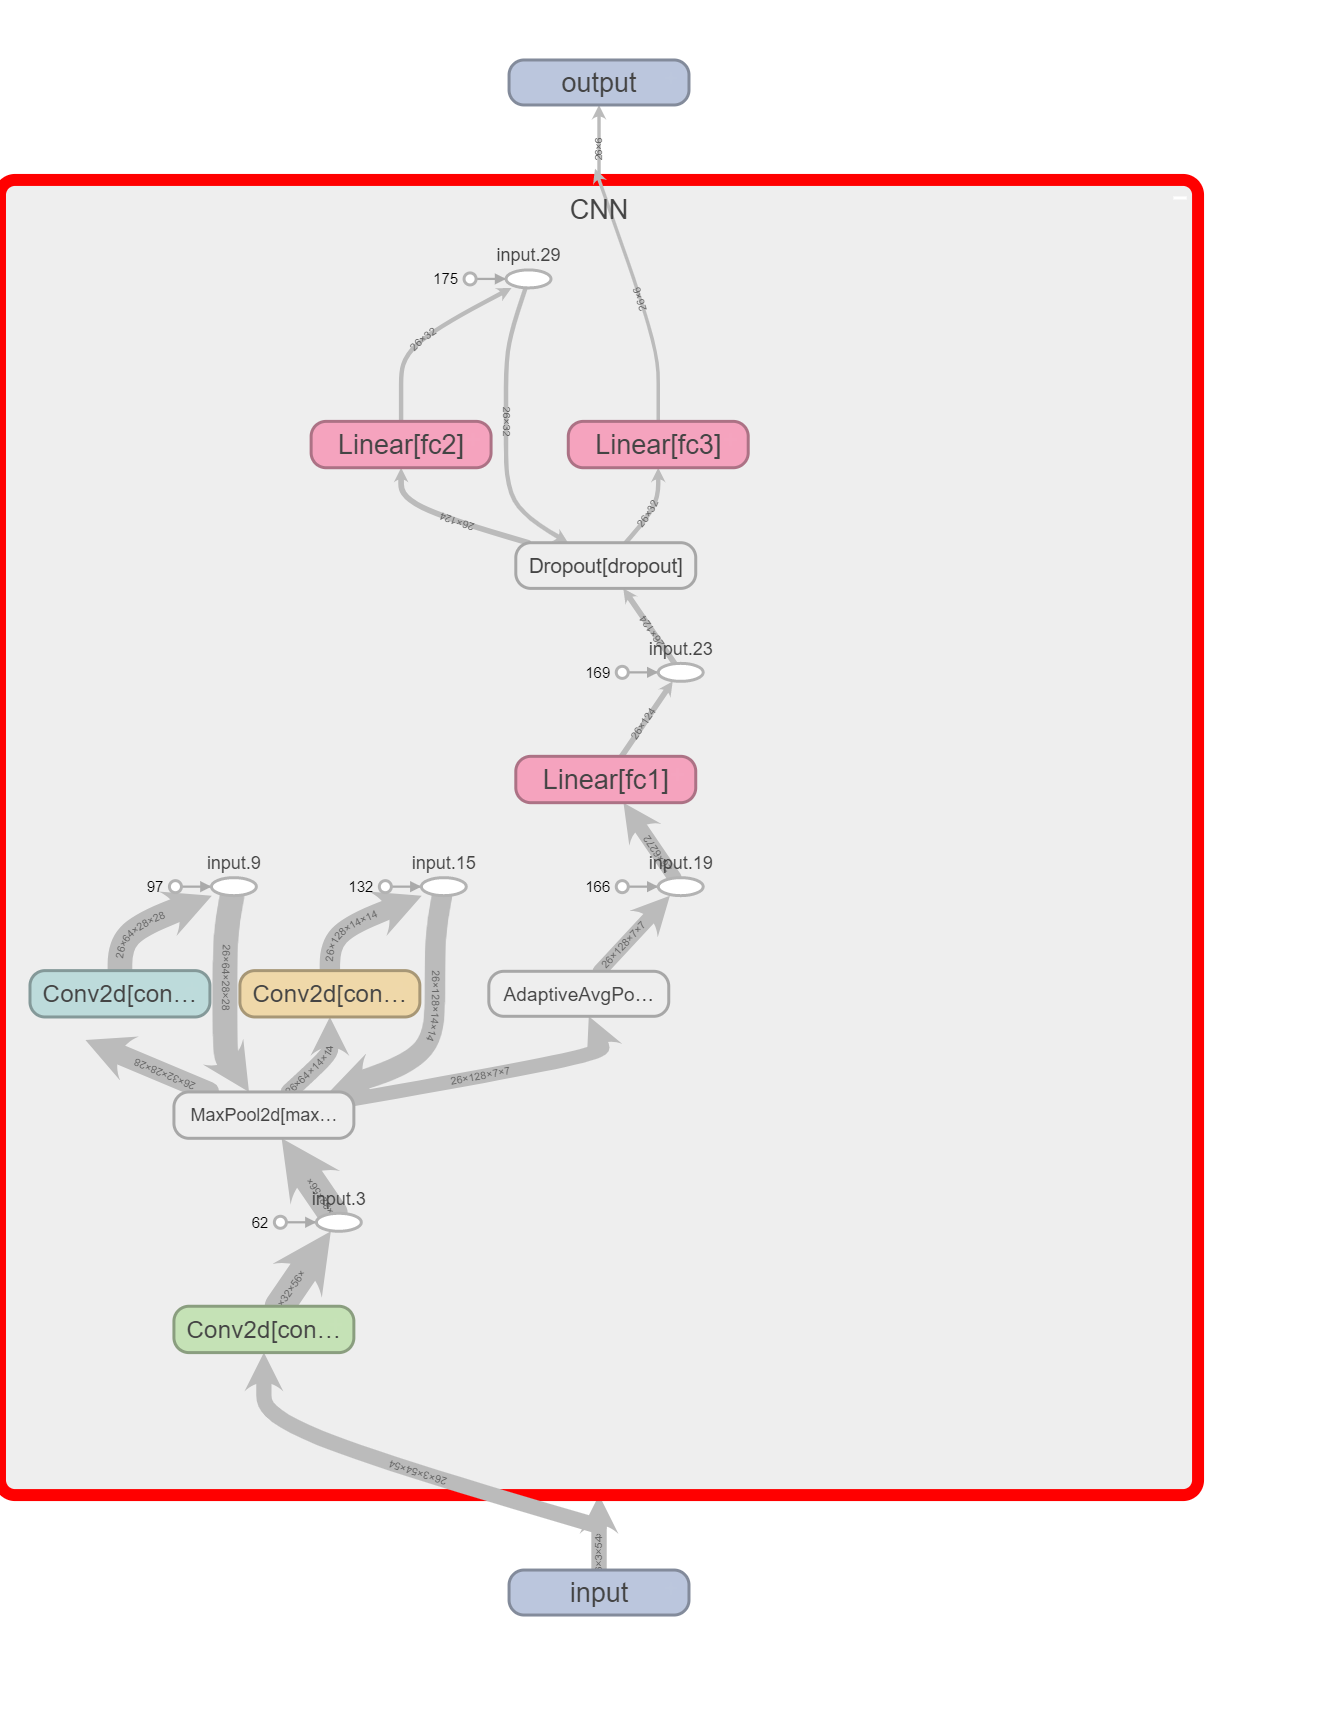
\includegraphics[scale = 0.2]{Img/Flowers/P1.png}
\end{figure}
\begin{python}
In [5]: class CNN(nn.Module):
          def __init__(self):
            super(CNN, self).__init__()
            self.maxpool = nn.MaxPool2d(kernel_size = 2, stride = 2)
            self.conv1 = nn.Conv2d(3,32,3,stride = 1, padding = 2)
            self.conv2 = nn.Conv2d(32,64,3,stride = 1, padding = 1)
            self.conv3 = nn.Conv2d(64,128,3,stride = 1, padding = 1)
            self.avgpool = nn.AdaptiveAvgPool2d((7, 7))
            self.dropout = nn.Dropout(p = 0.1)
            self.fc1 = nn.Linear(7*7*128, 124)
            self.fc2 = nn.Linear(124,32)
            self.fc3 = nn.Linear(32, 6)
            
          def forward(self, x):
            x = self.maxpool(F.leaky_relu(self.conv1(x)))
            x = self.maxpool(F.leaky_relu(self.conv2(x)))
            x = self.maxpool(F.leaky_relu(self.conv3(x)))
            x = self.avgpool(x)
            x = x.view(-1, 7*7*128)
            x = self.dropout(F.leaky_relu(self.fc1(x)))
            x = self.dropout(F.leaky_relu(self.fc2(x)))
            x = self.fc3(x)
            return x
        
        model = CNN().to(device)
        criterion = nn.CrossEntropyLoss()
        optimizer = torch.optim.Adam(model.parameters(), lr = learning_rate, weight_decay = weight_decay)
\end{python}
\newpage

\begin{python}
In [6]: from prettytable import PrettyTable
        
        def count_parameters(model):
            table = PrettyTable(["Modules", "Parameters"])
            total_params = 0
            for name, parameter in model.named_parameters():
                if not parameter.requires_grad: 
                    continue
                param = parameter.numel()
                table.add_row([name, param])
                total_params+=param
            print(table)
            print(f"Total Trainable Params: {total_params}")
            return total_params
        
        count_parameters(model)
\end{python}

\begin{minted}{bash}
        +--------------+------------+
        |   Modules    | Parameters |
        +--------------+------------+
        | conv1.weight |    864     |
        |  conv1.bias  |     32     |
        | conv2.weight |   18432    |
        |  conv2.bias  |     64     |
        | conv3.weight |   73728    |
        |  conv3.bias  |    128     |
        |  fc1.weight  |   777728   |
        |   fc1.bias   |    124     |
        |  fc2.weight  |    3968    |
        |   fc2.bias   |     32     |
        |  fc3.weight  |    192     |
        |   fc3.bias   |     6      |
        +--------------+------------+
        Total Trainable Params: 875298
Out [6]:875298
\end{minted}
\par - Tổng có 875298 tham số
\vspace{0.5 cm}

\par - Tiếp theo ta sẽ tiến hành train và đánh giá model

\newpage
\begin{python}
In [7]:
n_total_steps = len(train_loader)

run_loss = 0.0
run_acc = 0.0
for epoch in range(epochs):
    for i, (images, labels) in enumerate(tqdm(train_loader)):
        images = images.reshape(-1,3,54,54).to(device)
        labels = labels.to(device)
        _, labels = torch.max(labels.data, 1)

        outputs = model(images)
        loss = criterion(outputs,labels)
        
        run_loss +=loss.item() #for tensorboard
        _,pred = torch.max(outputs.data, 1)
        run_acc += (pred==labels).sum().item()#for tensorboard
        
        optimizer.zero_grad()
        loss.backward()
        optimizer.step()
        
        if (i+1) % 3 == 0:            
            with torch.no_grad():
                n_correct = 0
                n_samples = 0
                n_class_correct = [0 for i in range(5)]
                n_class_samples = [0 for i in range(5)]
                
                for images_val, labels_val in val_loader:
                    images_val = images_val.reshape(-1,3,54,54).to(device)
                    labels_val = labels_val.to(device)
                    _, labels_val = torch.max(labels_val.data, 1)
                    
                    output_val = model(images_val)
                    _, predict_val = torch.max(output_val.data, 1)
                    n_samples += labels_val.size(0)
                    n_correct += (predict_val == labels_val).sum().item()
                    loss_val = F.mse_loss(labels_val.float(),predict_val.float())
                    for i in range(26):
                        label_val = labels_val[i]
                        pred_val = predict_val[i]
                        if label_val == pred_val:
                            n_class_correct[label_val] += 1
                            
                        n_class_samples[label_val] += 1
                        
                acc_val = n_correct/(n_samples)
                run_acc_total = run_acc/((3-1)*128+pred.size(0))
                print(f'Epoch[{epoch+1}/{epochs}]:  Loss of Train: {(run_loss/3):.2f}, Accuracy of Train: {run_acc_total:.2f},Loss of Val: {loss_val:.2f} , Acc of Val: {acc_val:.2f}')
                      
print('Finished Training')
\end{python}

\begin{minted}{bash}
Out [7]:
100%[==========] 3/3 [00:06<00:00,  2.05s/it]
Epoch[1/80]:  Loss_Train: 1.67, Acc_Train: 0.32, Loss_Val: 1.54 , Acc_Val: 0.27
100%[==========] 3/3 [00:05<00:00,  1.85s/it]
Epoch[2/80]:  Loss_Train: 1.48, Acc_Train: 0.36, Loss_Val: 2.08 , Acc_Val: 0.38
100%[==========] 3/3 [00:05<00:00,  1.86s/it]
Epoch[3/80]:  Loss_Train: 1.39, Acc_Train: 0.35, Loss_Val: 2.27 , Acc_Val: 0.35
100%[==========] 3/3 [00:05<00:00,  1.79s/it]
Epoch[4/80]:  Loss_Train: 1.40, Acc_Train: 0.40, Loss_Val: 1.46 , Acc_Val: 0.69
100%[==========] 3/3 [00:05<00:00,  1.89s/it]
Epoch[5/80]:  Loss_Train: 1.30, Acc_Train: 0.45, Loss_Val: 1.65 , Acc_Val: 0.65
...
100%[==========] 3/3 [00:05<00:00,  1.78s/it]
Epoch[76/80]:  Loss_Train: 0.07, Acc_Train: 0.99, Loss_Val: 0.23 , Acc_Val: 0.88
100%[==========] 3/3 [00:05<00:00,  1.80s/it]
Epoch[77/80]:  Loss_Train: 0.09, Acc_Train: 0.98, Loss_Val: 0.42 , Acc_Val: 0.81
100%[==========] 3/3 [00:05<00:00,  1.80s/it]
Epoch[78/80]:  Loss_Train: 0.10, Acc_Train: 0.97, Loss_Val: 0.50 , Acc_Val: 0.92
100%[==========] 3/3 [00:05<00:00,  1.82s/it]
Epoch[79/80]:  Loss_Train: 0.06, Acc_Train: 0.98, Loss_Val: 0.73 , Acc_Val: 0.81
100%[==========] 3/3 [00:05<00:00,  1.72s/it]
Epoch[80/80]:  Loss_Train: 0.07, Acc_Train: 0.97, Loss_Val: 0.69 , Acc_Val: 0.85
Finished Training
\end{minted}


\begin{python}
In [8]: with torch.no_grad():
            n_correct = 0
            n_samples = 0
            n_class_correct = [0 for i in range(5)]
            n_class_samples = [0 for i in range(5)]
            
            for images, labels in val_loader:
                images = images.reshape(-1,3,54,54).to(device)
                labels = labels.to(device)
                _, labels = torch.max(labels.data, 1)
                output = model(images)
                
                _, predict = torch.max(output.data, 1)
                n_samples += labels.size(0)
                n_correct += (predict == labels).sum().item()
                
                for i in range(26):
                    label = labels[i]
                    pred = predict[i]
                    if label == pred:
                        n_class_correct[label] +=1
                        
                    n_class_samples[label]+=1
            acc = 100.0*n_correct/n_samples
            print(f'Accuracy of the network: {acc} %')
\end{python}

\begin{minted}{bash}
Out [8]: Accuracy of the network: 96.15384615384616 %
\end{minted}
\par- Sau 80 epochs ta có thể thấy độ chính xác trên tập validation là 96 $\%$
\par- Dưới dây là dồ thị của độ chính xác. Màu cam của tập train và màu tím của tập validation.
Chi tiết xem thêm tại đây [12]

\begin{figure}[h] %% [h] --> here
    \centering
    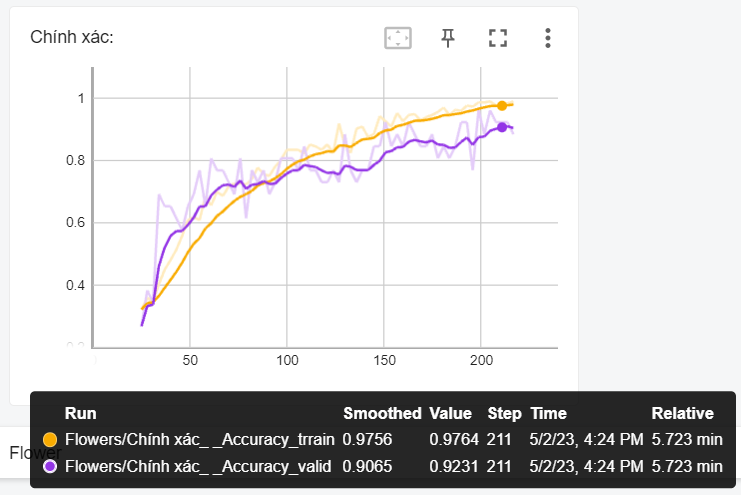
\includegraphics[scale = 0.6]{Img/Flowers/P2.png}
\end{figure}

\par - Dưới dây là dồ thị của độ mất mát. Màu hồng của tập train và màu xanh của tập validation. Chi tiết xem thêm tại đây [12]
\begin{figure}[h] %% [h] --> here
    \centering
    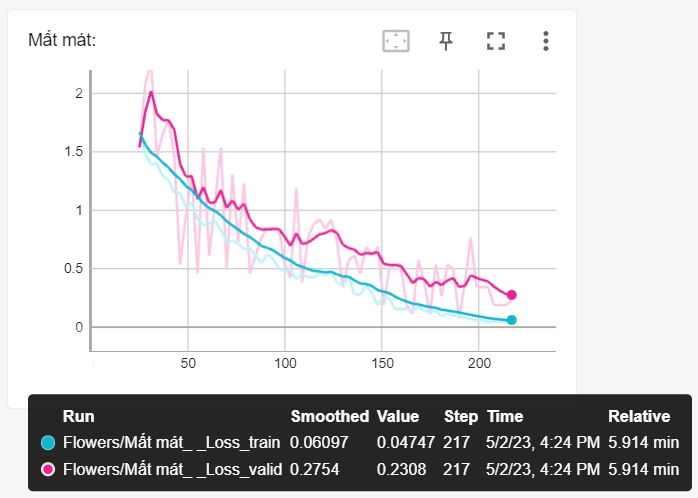
\includegraphics[scale = 0.65]{Img/Flowers/P3.png}
\end{figure}
\par - Tiến hành lưu và load model 

\begin{python}
In [9]:# Save model
        FILE = "model.pth"
        torch.save(model.state_dict(), FILE)
        # Load model
        loaded_model = CNN().to(device)
        loaded_model.load_state_dict(torch.load(FILE)) 
        loaded_model.eval()
\end{python}
\newpage
\begin{minted}{bash}
Out [9]:
    CNN(
      (maxpool): MaxPool2d(kernel_size=2, stride=2, padding=0, dilation=1, 
                            ceil_mode=False)
      (conv1): Conv2d(3, 32, kernel_size=(3, 3), stride=(1, 1), padding=(2, 2))
      (conv2): Conv2d(32, 64, kernel_size=(3, 3), stride=(1, 1), padding=(1, 1))
      (conv3): Conv2d(64, 128, kernel_size=(3, 3), stride=(1, 1), padding=(1, 1))
      (avgpool): AdaptiveAvgPool2d(output_size=(7, 7))
      (dropout): Dropout(p=0.1, inplace=False)
      (fc1): Linear(in_features=6272, out_features=124, bias=True)
      (fc2): Linear(in_features=124, out_features=32, bias=True)
      (fc3): Linear(in_features=32, out_features=6, bias=True)
    )
\end{minted}
\par - Cuối cùng ta tiến hành thử nghiệm model với ảnh từ tập test.
\begin{python}
In [10]:from torchvision import transforms
        import PIL.Image as Image
        
        url = '/kaggle/input/flower-s/FLOWERS/Test/Daisy.jpg'
        # Load anh
        img = Image.open(url)
        
        # Hien thi anh
        plt.imshow(img)
        plt.show()
        # Ap dung transform
        
        img_transformed = transform(img)
        
        test = loaded_model(img_transformed.to(device))
        print(class_name[torch.max(test.data,1)[1].data])
\end{python}
\begin{figure}[h] %% [h] --> here
    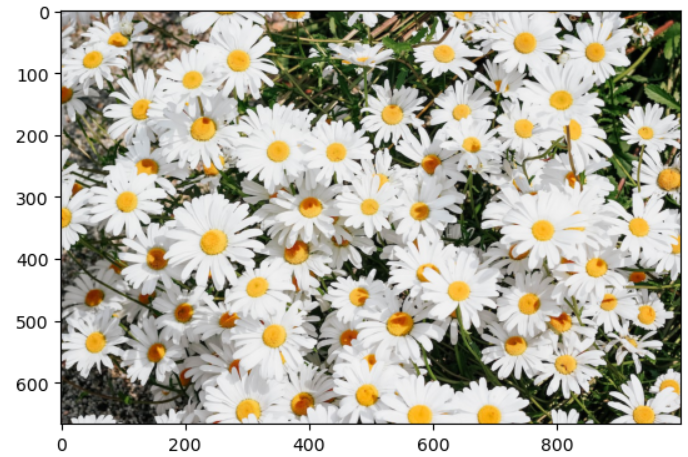
\includegraphics[scale = 0.65]{Img/Flowers/P4.png}
\end{figure}
\begin{minted}{bash}
Out [10]: Daisy
\end{minted}
















\newpage
\subsection{10 Vietnamese dishes (bún bò, chè, bánh xèo......)}
\par \textbf{Code đầy đủ ở đây [8]}
\par\hspace{0cm}- Đầu tiên ta sẽ import các thư viện cần thiết cho việc xây dựng và thực thi model
\par\hspace{0cm}- Ở đây ta sẽ dùng Cuda cho việc xây model trên GPU và nó giúp ta tăng tống quá trình train và thực thi model

\begin{python}
In [1]: import numpy as np
        from tqdm import tqdm
        import torch
        import torch.nn as nn
        import torchvision
        import torch.nn.functional as F
        from torch.utils.data import DataLoader
        from torchvision import datasets, transforms, models
        from torchvision.transforms import ToTensor
        import matplotlib.pyplot as plt
        from torch.utils.tensorboard import SummaryWriter
        
        
        device = torch.device('cuda' if torch.cuda.is_available() else 'cpu')
        print(device)

\end{python}
\begin{minted}{bash}
Out [1]: cuda
\end{minted}

\par - Tiếp Theo ta sẽ xây dựng hàm transform để biến đổi trên dữ liệu (data augmentation) hoặc chuẩn hóa (data normalization) dữ liệu trước khi đưa vào huấn luyện mô hình.
\par - Việc sử dụng hàm transform giúp cho mô hình huấn luyện được đào tạo trên nhiều dữ liệu
đa dạng hơn, giúp mô hình học được các đặc trưng tổng quát hơn và tránh overfitting trên dữ liệu huấn luyện.
\par - Quy trình của hàm transform: Thay đổi kích thước ảnh về dạng (224x224) $\Rightarrow$ Chuyển về dạng tensor $\Rightarrow$ Chuẩn hóa ma trận.

\begin{python}
In [2]: transform = transforms.Compose([
                transforms.RandomRotation(10),      
                transforms.RandomHorizontalFlip(),  
                transforms.Resize(244),             
                transforms.CenterCrop(244),         
                transforms.ToTensor(),
                transforms.Normalize([0.485, 0.456, 0.406],
                                     [0.229, 0.224, 0.225])
        ])
        
        class FoodDataset(torch.utils.data.Dataset):
            def __init__(self, root, transform = None):
                self.data = datasets.ImageFolder(root, transform = transform)
                self.classes = self.data.classes
                self.num_classes = len(self.classes)
            def __getitem__(self, index):
                img, label = self.data[index]
                one_hot_label = F.one_hot(torch.tensor(label), num_classes=self.num_classes).float()
                return img, one_hot_label   
            
            def __len__(self):
                    return len(self.data)
                
        x_train = FoodDataset( root=("/kaggle/input/vn-food/Food/Train"), transform = transform)
        x_val = FoodDataset(root = ('/kaggle/input/vn-food/Food/Val'), transform = transform)
\end{python}

\par - Tiếp theo ta sẽ tiến hành thiết lập siêu tham số (hyperparameter) và chia dữ liệu theo batch
cho model
\par - Ở đây ta sử dụng Weight Decay (L2 Regularization) bằng 0.0001 để giảm thiểu Overfitting [5]
\begin{python}
In [3]: class_name = x_train.classes
        print("Tong class: ",len(class_name))
        print("Ten cac loai: ",class_name)
        
        batch = 128
        epochs = 80
        learning_rate = 1e-3
        weight_decay = 1e-4
        
        train_loader = DataLoader(x_train, batch_size = batch, shuffle = True)
        val_loader = DataLoader(x_val, batch_size = batch, shuffle = True)
        
        
        examples = iter(val_loader)
        example_data, example_targets = next(examples)
\end{python}

\begin{minted}{bash}
Out [3]: Tong class:  10
        Ten cac loai:  ['Banh bot loc', 'Banh chung', 'Banh khot', 'Banh mi', 
                        'Banh trang nuong', 'Bun bo Hue', 'Bun thit nuong', 
                        'Chao long', 'Com tam', 'Xoi xeo']    
\end{minted}
\newpage
\par - Tiếp theo ta sẽ tiến hành xây dựng model CNN
\par - Dưới đây là hình ảnh cấu trúc model CNN. Chi tiết xem thêm tại đây[13]

\begin{figure}[h] %% [h] --> here
    \centering
    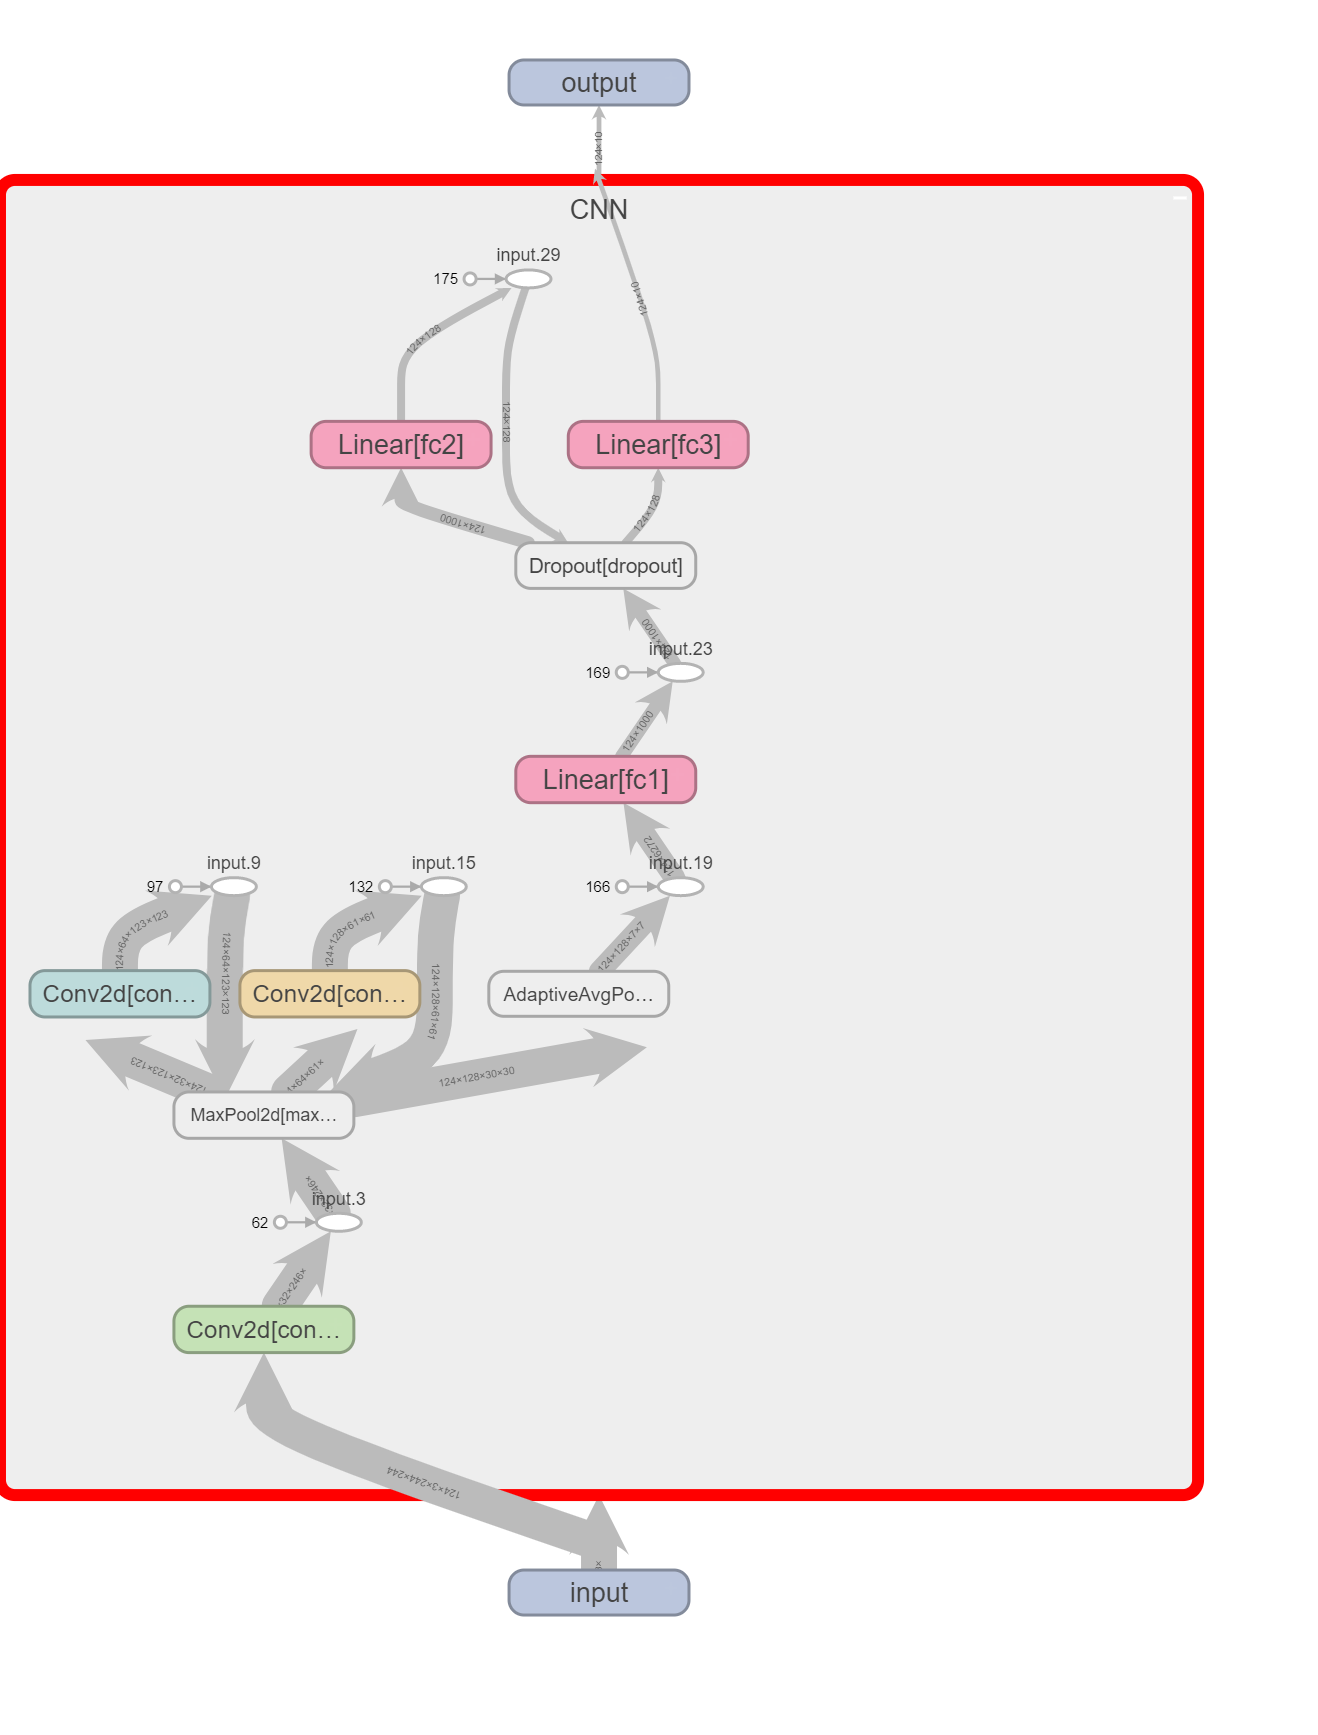
\includegraphics[scale = 0.2]{Img/Dishes/P1.png}
\end{figure}

\begin{python}
In [4]: class CNN(nn.Module):
          def __init__(self):
            super(CNN, self).__init__()
            self.maxpool = nn.MaxPool2d(kernel_size = 2, stride = 2)
            self.conv1 = nn.Conv2d(3,32,3,stride = 1, padding = 2)
            self.conv2 = nn.Conv2d(32,64,3,stride = 1, padding = 1)
            self.conv3 = nn.Conv2d(64,128,3,stride = 1, padding = 1)
            self.avgpool = nn.AdaptiveAvgPool2d((7, 7))
            self.dropout = nn.Dropout(p = 0.5)
            self.fc1 = nn.Linear(7*7*128, 1000)
            self.fc2 = nn.Linear(1000,128)
            self.fc3 = nn.Linear(128, 10)
          def forward(self, x):
            x = self.maxpool(F.leaky_relu(self.conv1(x)))
            x = self.maxpool(F.leaky_relu(self.conv2(x)))
            x = self.maxpool(F.leaky_relu(self.conv3(x)))
            x = self.avgpool(x)
            x = x.view(-1, 7*7*128)
            x = self.dropout(F.leaky_relu(self.fc1(x)))
            x = self.dropout(F.leaky_relu(self.fc2(x)))
            x = self.fc3(x)
            return x
        
        model = CNN().to(device)
        criterion = nn.CrossEntropyLoss()
        optimizer = torch.optim.Adam(model.parameters(), lr = learning_rate, weight_decay = weight_decay)
\end{python}

\begin{python}
In [7]:from prettytable import PrettyTable
        
        def count_parameters(model):
            table = PrettyTable(["Modules", "Parameters"])
            total_params = 0
            for name, parameter in model.named_parameters():
                if not parameter.requires_grad: 
                    continue
                param = parameter.numel()
                table.add_row([name, param])
                total_params+=param
            print(table)
            print(f"Total Trainable Params: {total_params}")
            return total_params
        
        count_parameters(model)
\end{python}
\begin{minted}{bash}
    +--------------+------------+
    |   Modules    | Parameters |
    +--------------+------------+
    | conv1.weight |    864     |
    |  conv1.bias  |     32     |
    | conv2.weight |   18432    |
    |  conv2.bias  |     64     |
    | conv3.weight |   73728    |
    |  conv3.bias  |    128     |
    |  fc1.weight  |  6272000   |
    |   fc1.bias   |    1000    |
    |  fc2.weight  |   128000   |
    |   fc2.bias   |    128     |
    |  fc3.weight  |    1280    |
    |   fc3.bias   |     10     |
    +--------------+------------+
    Total Trainable Params: 6495666
Out [7]: 6495666
\end{minted}
\par - Tổng có 6495666 tham số
\vspace{0.5cm}
\par - Tiếp theo ta sẽ tiến hành train và đánh giá model
\newpage
\begin{python}
In [8]:
n_total_steps = len(train_loader)

run_loss = 0.0
run_acc = 0.0
for epoch in range(epochs):
    for i, (images, labels) in enumerate(tqdm(train_loader)):
        images = images.reshape(-1,3,244,244).to(device)
        labels = labels.to(device)
        _, labels = torch.max(labels.data, 1)
        outputs = model(images)
        loss = criterion(outputs,labels)
        
        run_loss +=loss.item() #for tensorboard
        _,pred = torch.max(outputs.data, 1)
        run_acc += (pred==labels).sum().item()#for tensorboard
        
        optimizer.zero_grad()
        loss.backward()
        optimizer.step()
        
        if (i+1) % 3 == 0:   
            with torch.no_grad():
                n_correct = 0
                n_samples = 0
                n_class_correct = [0 for i in range(10)]
                n_class_samples = [0 for i in range(10)]
                
                for images_val, labels_val in val_loader:
                    images_val = images_val.reshape(-1,3,244,244).to(device)
                    labels_val = labels_val.to(device)
                    _, labels_val = torch.max(labels_val.data, 1)
                    
                    output_val = model(images_val)
                    _, predict_val = torch.max(output_val.data, 1)
                    n_samples += labels_val.size(0)
                    n_correct += (predict_val == labels_val).sum().item()
                    loss_val = F.mse_loss(labels_val.float(),predict_val.float())
                    for i in range(26):
                        label_val = labels_val[i]
                        pred_val = predict_val[i]
                        if label_val == pred_val:
                            n_class_correct[label_val] += 1
                            
                        n_class_samples[label_val] += 1
                       
                acc_val = n_correct/(n_samples)
                acc_val_total = run_acc/((3-1)*128+pred.size(0))

                print(f'Epoch[{epoch+1}/{epochs}]:  Loss_Train: {(run_loss/3):.2f}, Acc_Train: {acc_val_total:.2f} , Loss_Val: {loss_val:.2f} , Acc_Val: {acc_val:.2f}')
            
print('Finished Training')
\end{python}

\begin{minted}{bash}
Out [8]:
100%[==========] 3/3 [00:12<00:00,  4.16s/it]
Epoch[1/80]:  Loss_Train: 2.32, Acc_Train: 0.10 , Loss_Val: 12.56 , Acc_Val: 0.13
100%[==========] 3/3 [00:11<00:00,  3.98s/it]
Epoch[2/80]:  Loss_Train: 2.29, Acc_Train: 0.12 , Loss_Val: 13.07 , Acc_Val: 0.14
100%[==========] 3/3 [00:11<00:00,  3.86s/it]
Epoch[3/80]:  Loss_Train: 2.27, Acc_Train: 0.15 , Loss_Val: 12.53 , Acc_Val: 0.19
100%[==========] 3/3 [00:11<00:00,  3.80s/it]
Epoch[4/80]:  Loss_Train: 2.20, Acc_Train: 0.22 , Loss_Val: 15.38 , Acc_Val: 0.21
100%[==========] 3/3 [00:11<00:00,  3.91s/it]
Epoch[5/80]:  Loss_Train: 2.16, Acc_Train: 0.18 , Loss_Val: 14.32 , Acc_Val: 0.21
...
100%[==========] 3/3 [00:11<00:00,  3.85s/it]
Epoch[76/80]:  Loss_Train: 0.12, Acc_Train: 0.96 , Loss_Val: 1.44 , Acc_Val: 0.90
100%[==========] 3/3 [00:11<00:00,  3.86s/it]
Epoch[77/80]:  Loss_Train: 0.05, Acc_Train: 0.99 , Loss_Val: 1.93 , Acc_Val: 0.86
100%[==========] 3/3 [00:11<00:00,  3.94s/it]
Epoch[78/80]:  Loss_Train: 0.12, Acc_Train: 0.97 , Loss_Val: 3.54 , Acc_Val: 0.82
100%[==========] 3/3 [00:11<00:00,  3.83s/it]
Epoch[79/80]:  Loss_Train: 0.11, Acc_Train: 0.96 , Loss_Val: 2.65 , Acc_Val: 0.81
100%[==========] 3/3 [00:11<00:00,  3.84s/it]
Epoch[80/80]:  Loss_Train: 0.11, Acc_Train: 0.97 , Loss_Val: 3.52 , Acc_Val: 0.82
Finished Training

\end{minted}
\begin{python}
In [9]: with torch.no_grad():
            n_correct = 0
            n_samples = 0
            n_class_correct = [0 for i in range(10)]
            n_class_samples = [0 for i in range(10)]   
            for images, labels in val_loader:
                images = images.reshape(-1,3,244,244).to(device)
                labels = labels.to(device)
                _, labels = torch.max(labels.data, 1)
                output = model(images)  
                _, predict = torch.max(output.data, 1)
                n_samples += labels.size(0)
                n_correct += (predict == labels).sum().item() 
                for i in range(87):
                    label = labels[i]
                    pred = predict[i]
                    if label == pred:
                        n_class_correct[label] +=1
                        
                    n_class_samples[label]+=1       
            acc = 100.0*n_correct/n_samples
            print(f'Accuracy of the network: {acc} %')
\end{python}
\begin{minted}{bash}
Out [8]: Accuracy of the network: 83.06451612903226 %
    
\end{minted}
\par- Sau 80 epochs ta có thể thấy độ chính xác trên tập validation là 83 $\%$
\par- Dưới dây là dồ thị của độ chính xác. Màu xanh đen của tập train và màu xanh sáng của tập validation.
Chi tiết xem thêm tại đây [13]

\begin{figure}[h] %% [h] --> here
    \centering
    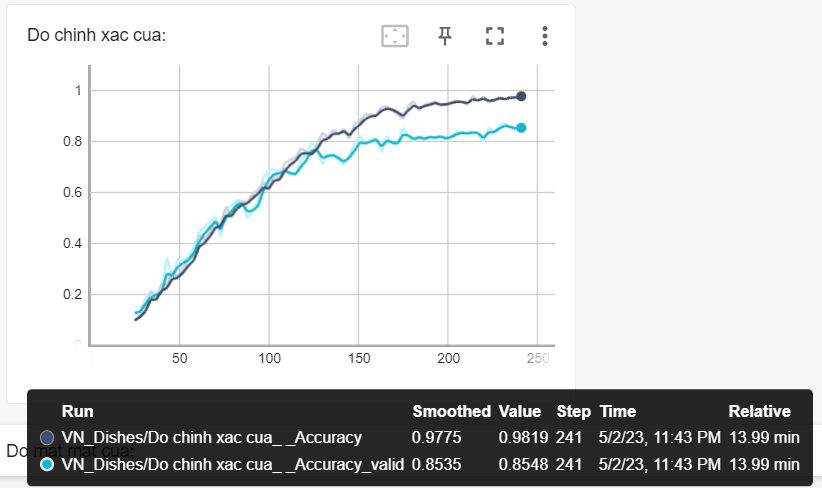
\includegraphics[scale = 0.6]{Img/Dishes/P2.png}
\end{figure}

\par - Dưới dây là dồ thị của độ mất mát. Màu cam của tập train và màu xanh lá của tập validation. Chi tiết xem thêm tại đây [13]
\begin{figure}[h] %% [h] --> here
    \centering
    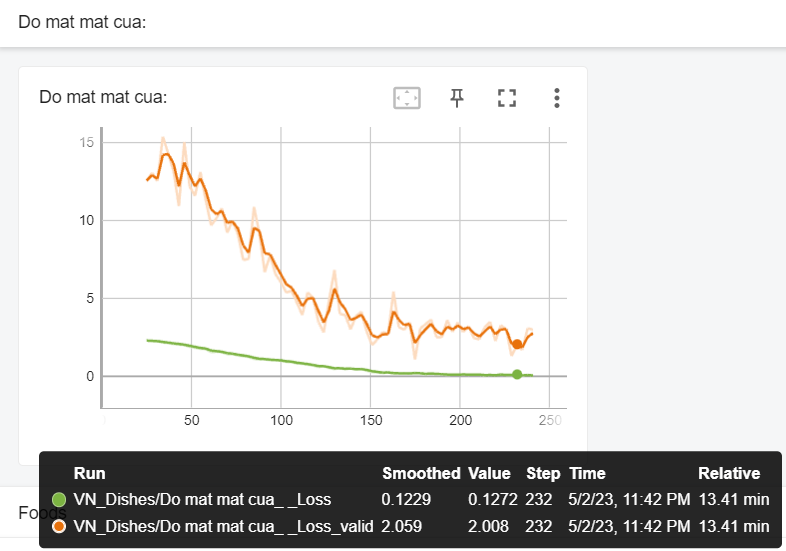
\includegraphics[scale = 0.65]{Img/Dishes/P3.png}
\end{figure}
\par - Tiến hành lưu và load model 

\begin{python}
In [9]:# Save model
        FILE = "model.pth"
        torch.save(model.state_dict(), FILE)
        # Load model
        loaded_model = CNN().to(device)
        loaded_model.load_state_dict(torch.load(FILE)) 
        loaded_model.eval()
\end{python}
\newpage
\begin{minted}{bash}
Out [9]:CNN(
          (maxpool): MaxPool2d(kernel_size=2, stride=2, padding=0, dilation=1, 
                                ceil_mode=False)
          (conv1): Conv2d(3, 32, kernel_size=(3, 3), stride=(1, 1), padding=(2, 2))
          (conv2): Conv2d(32, 64, kernel_size=(3, 3), stride=(1, 1), padding=(1, 1))
          (conv3): Conv2d(64, 128, kernel_size=(3, 3), stride=(1, 1), padding=(1, 1))
          (avgpool): AdaptiveAvgPool2d(output_size=(7, 7))
          (dropout): Dropout(p=0.5, inplace=False)
          (fc1): Linear(in_features=6272, out_features=1000, bias=True)
          (fc2): Linear(in_features=1000, out_features=128, bias=True)
          (fc3): Linear(in_features=128, out_features=10, bias=True)
        )    
\end{minted}
\par - Cuối cùng ta tiến hành thử nghiệm model với ảnh từ tập test.
\begin{python}
In [10]:from torchvision import transforms
        import PIL.Image as Image
        url = '/kaggle/input/vn-food/Food/Test/comtam.jpg'
        
        # Load anh
        img = Image.open(url)
        # Hien thi anh
        plt.imshow(img)
        plt.show()
        
        # Ap dung transform
        img_transformed = transform(img)
        test = loaded_model(img_transformed.to(device))
        print(class_name[torch.max(test.data,1)[1].data])
\end{python}
\begin{figure}[h] %% [h] --> here
    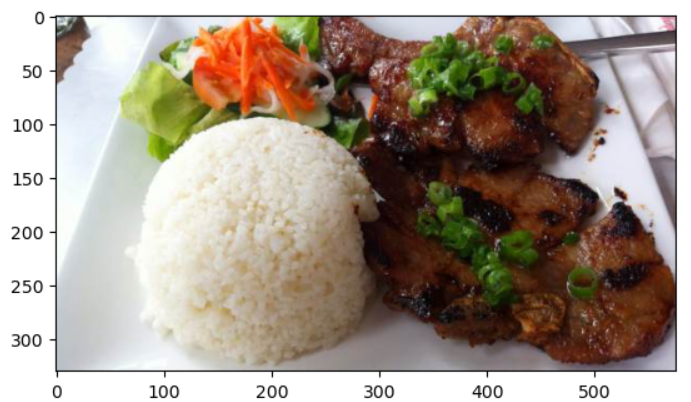
\includegraphics[scale = 0.7]{Img/Dishes/P5.png}
\end{figure}

\begin{minted}{bash}
Out[10]:Com tam
\end{minted}








\newpage
\subsection{VN banknotes (5000vnd, 10000vnd, 20k, 50k, 100k, 500k)}
\par \textbf{Code đầy đủ ở đây [9]}
\par\hspace{0cm}- Đầu tiên ta sẽ import các thư viện cần thiết cho việc xây dựng và thực thi model
\par\hspace{0cm}- Ở đây ta sẽ dùng Cuda cho việc xây model trên GPU và nó giúp ta tăng tống quá trình train và thực thi model
\begin{python}
In [1]: import numpy as np
        from tqdm import tqdm
        import torch
        import torch.nn as nn
        import torchvision
        import torch.nn.functional as F
        from torch.utils.data import DataLoader
        from torchvision import datasets, transforms, models
        from torchvision.transforms import ToTensor
        import matplotlib.pyplot as plt
        from torch.utils.tensorboard import SummaryWriter
        
        
        device = torch.device('cuda' if torch.cuda.is_available() else 'cpu')
        print(device)
\end{python}
\begin{minted}{bash}
Out [1]: cuda
\end{minted}
\par - Tiếp Theo ta sẽ xây dựng hàm transform để biến đổi trên dữ liệu (data augmentation) hoặc chuẩn hóa (data normalization) dữ liệu trước khi đưa vào huấn luyện mô hình.
\par - Việc sử dụng hàm transform giúp cho mô hình huấn luyện được đào tạo trên nhiều dữ liệu
đa dạng hơn, giúp mô hình học được các đặc trưng tổng quát hơn và tránh overfitting trên dữ liệu huấn luyện.
\par - Quy trình của hàm transform: Thay đổi kích thước ảnh về dạng (64x64) $\Rightarrow$ Chuyển về dạng tensor $\Rightarrow$ Chuẩn hóa ma trận.

\begin{python}
In [2]: transform = transforms.Compose([
                transforms.RandomRotation(10),      
                transforms.RandomHorizontalFlip(),  
                transforms.Resize((64,64)),             
                transforms.ToTensor(),
                transforms.Normalize([0.485, 0.456, 0.406],
                                     [0.229, 0.224, 0.225])
        ])
        
        class MoneyDataset(torch.utils.data.Dataset):
            def __init__(self, root, transform = None):
                self.data = datasets.ImageFolder(root, transform = transform)
                self.classes = self.data.classes
                self.num_classes = len(self.classes)
            def __getitem__(self, index):
                img, label = self.data[index]
                one_hot_label = F.one_hot(torch.tensor(label), num_classes=self.num_classes).float()
                return img, one_hot_label   
            
            def __len__(self):
                    return len(self.data)
                
        x_train = MoneyDataset( root=("/kaggle/input/vn-money/Money/Train"), transform = transform)
        x_val = MoneyDataset(root = ('/kaggle/input/vn-money/Money/Val'), transform = transform)
\end{python}
\par - Tiếp theo ta sẽ tiến hành thiết lập siêu tham số (hyperparameter) và chia dữ liệu theo batch
cho model
\par - Ở đây ta sử dụng Weight Decay (L2 Regularization) bằng 0.0001 để giảm thiểu Overfitting [5]

\begin{python}
In [3]: class_name = x_train.classes
        print("Tong class: ",len(class_name))
        print("Ten cac loai: ",class_name)
        
        batch = 128
        epochs = 80
        learning_rate = 3*1e-3
        weight_decay = 1e-4
        
        train_loader = DataLoader(x_train, batch_size = batch, shuffle = True)
        val_loader = DataLoader(x_val, batch_size = batch, shuffle = True)
        
        
        examples = iter(val_loader)
        example_data, example_targets = next(examples)
\end{python}

\begin{minted}{bash}
Out [3]: Tong class:  6
         Ten cac loai:  ['100k', '10k', '20k', '500k', '50k', '5k'] 
\end{minted}

\newpage
\par - Tiếp theo ta sẽ tiến hành xây dựng model CNN
\par - Dưới đây là hình ảnh cấu trúc model CNN. Chi tiết xem thêm tại đây[14]

\begin{figure}[h] %% [h] --> here
    \centering
    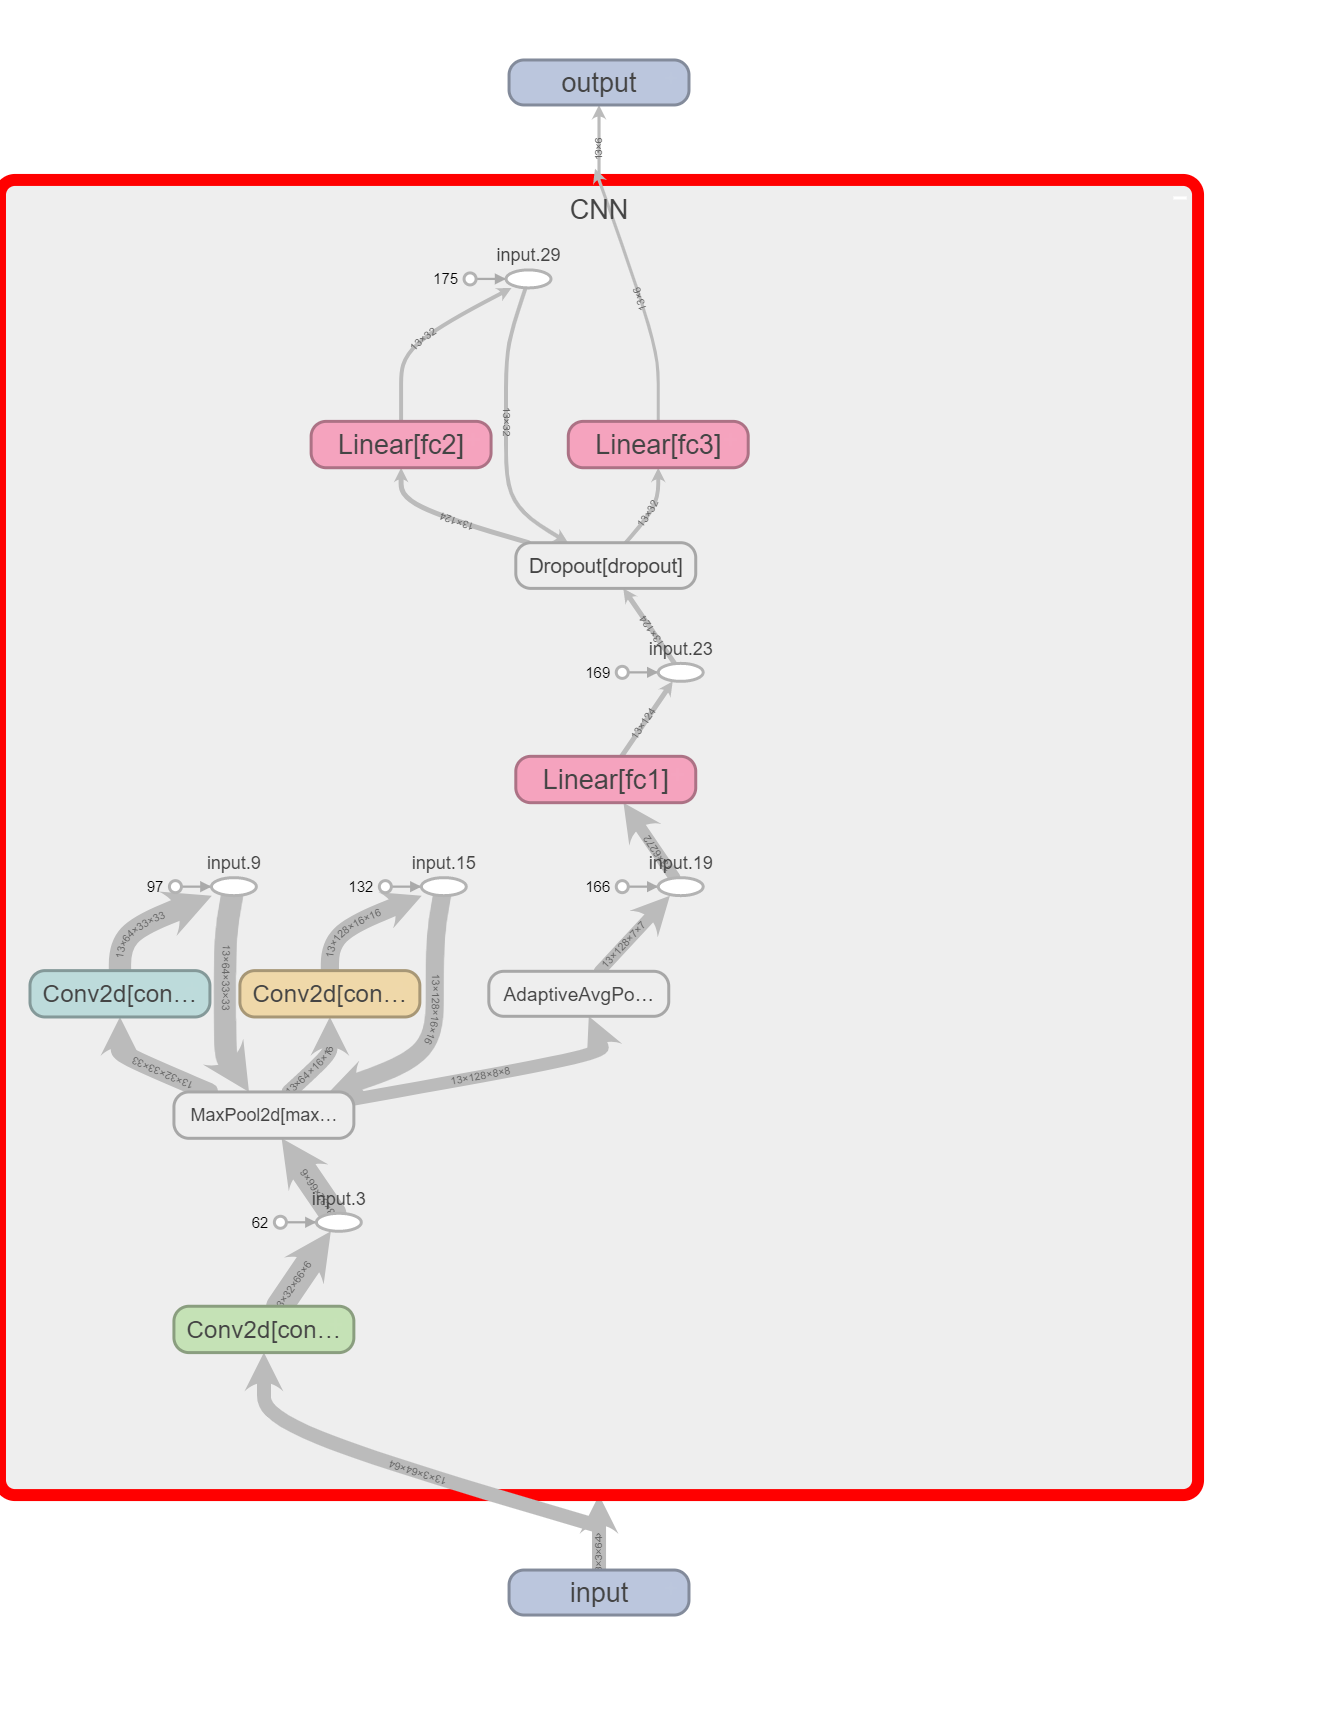
\includegraphics[scale = 0.2]{Img/Money/P1.png}
\end{figure}

\begin{python}
In [4]: class CNN(nn.Module):
          def __init__(self):
            super(CNN, self).__init__()
            self.maxpool = nn.MaxPool2d(kernel_size = 2, stride = 2)
            self.conv1 = nn.Conv2d(3,32,3,stride = 1, padding = 2)
            self.conv2 = nn.Conv2d(32,64,3,stride = 1, padding = 1)
            self.conv3 = nn.Conv2d(64,128,3,stride = 1, padding = 1)
            self.avgpool = nn.AdaptiveAvgPool2d((7, 7))
            self.dropout = nn.Dropout(p = 0.1)
            self.fc1 = nn.Linear(7*7*128, 124)
            self.fc2 = nn.Linear(124,32)
            self.fc3 = nn.Linear(32, 6) 
          def forward(self, x):
            x = self.maxpool(F.leaky_relu(self.conv1(x)))
            x = self.maxpool(F.leaky_relu(self.conv2(x)))
            x = self.maxpool(F.leaky_relu(self.conv3(x)))
            x = self.avgpool(x)
            x = x.view(-1, 7*7*128)
            x = self.dropout(F.leaky_relu(self.fc1(x)))
            x = self.dropout(F.leaky_relu(self.fc2(x)))
            x = self.fc3(x)
            return x
        model = CNN().to(device)
        criterion = nn.CrossEntropyLoss()
        optimizer = torch.optim.Adam(model.parameters(), lr = learning_rate, weight_decay = weight_decay)
\end{python}
\begin{python}
In [5]: from prettytable import PrettyTable
    
        def count_parameters(model):
            table = PrettyTable(["Modules", "Parameters"])
            total_params = 0
            for name, parameter in model.named_parameters():
                if not parameter.requires_grad: 
                    continue
                param = parameter.numel()
                table.add_row([name, param])
                total_params+=param
            print(table)
            print(f"Total Trainable Params: {total_params}")
            return total_params
        
        count_parameters(model)
\end{python}
\begin{minted}{bash}
+--------------+------------+
|   Modules    | Parameters |
+--------------+------------+
| conv1.weight |    864     |
|  conv1.bias  |     32     |
| conv2.weight |   18432    |
|  conv2.bias  |     64     |
| conv3.weight |   73728    |
|  conv3.bias  |    128     |
|  fc1.weight  |   777728   |
|   fc1.bias   |    124     |
|  fc2.weight  |    3968    |
|   fc2.bias   |     32     |
|  fc3.weight  |    192     |
|   fc3.bias   |     6      |
+--------------+------------+
Total Trainable Params: 875298
Out [5]: 875298
\end{minted}

\par - Tổng có 875298 tham số
\vspace{0.5cm}
\par - Tiếp theo ta sẽ tiến hành train và đánh giá model
\newpage

\begin{python}
In [6]:
n_total_steps = len(train_loader)
run_loss = 0.0
run_acc = 0.0
for epoch in range(epochs):
    for i, (images, labels) in enumerate(tqdm(train_loader)):
        images = images.reshape(-1,3,64,64).to(device)
        labels = labels.to(device)
        _, labels = torch.max(labels.data, 1)
        outputs = model(images)
        loss = criterion(outputs,labels)
        run_loss +=loss.item() #for tensorboard
        _,pred = torch.max(outputs.data, 1)
        run_acc += (pred==labels).sum().item()#for tensorboard
        
        optimizer.zero_grad()
        loss.backward()
        optimizer.step()
        
        if (i+1) % 3 == 0:
            with torch.no_grad():
                n_correct = 0
                n_samples = 0
                n_class_correct = [0 for i in range(6)]
                n_class_samples = [0 for i in range(6)]
                
                for images_val, labels_val in val_loader:
                    images_val = images_val.reshape(-1,3,64,64).to(device)
                    labels_val = labels_val.to(device)
                    _, labels_val = torch.max(labels_val.data, 1)
                    
                    output_val = model(images_val)
                    _, predict_val = torch.max(output_val.data, 1)
                    n_samples += labels_val.size(0)
                    n_correct += (predict_val == labels_val).sum().item()
                    loss_val = F.mse_loss(labels_val.float(),predict_val.float())
                    for i in range(13):
                        label_val = labels_val[i]
                        pred_val = predict_val[i]
                        if label_val == pred_val:
                            n_class_correct[label_val] += 1
                            
                        n_class_samples[label_val] += 1
                        
                acc_val = n_correct/(n_samples)
                acc_total = run_acc/((3-1)*128+pred.size(0))
                print(f'Epoch[{epoch+1}/{epochs}]: Loss_Train: {(run_loss/3):.2f}, Acc_Train: {acc_total:.2f} , Loss_Val: {loss_val:.2f} , Acc_Val: {acc_val:.2f} ')
print('Finished Training')
\end{python}
\newpage
\begin{minted}{bash}
Out [6]:
100%[==========] 3/3 [00:01<00:00,  2.07it/s]
Epoch[1/80]: Loss_Train: 1.73, Acc_Train: 0.41 , Loss_Val: 4.85 , Acc_Val: 0.15 
100%[==========] 3/3 [00:01<00:00,  2.37it/s]
Epoch[2/80]: Loss_Train: 1.49, Acc_Train: 0.52 , Loss_Val: 10.38 , Acc_Val: 0.15
100%[==========] 3/3 [00:01<00:00,  2.27it/s]
Epoch[3/80]: Loss_Train: 1.11, Acc_Train: 0.75 , Loss_Val: 10.38 , Acc_Val: 0.15 
100%[==========] 3/3 [00:01<00:00,  2.17it/s]
Epoch[4/80]: Loss_Train: 0.85, Acc_Train: 0.73 , Loss_Val: 8.08 , Acc_Val: 0.31 
100%[==========] 3/3 [00:01<00:00,  2.19it/s]
Epoch[5/80]: Loss_Train: 0.69, Acc_Train: 0.74 , Loss_Val: 4.38 , Acc_Val: 0.31 
...
Epoch[76/80]: Loss_Train: 0.02, Acc_Train: 0.99 , Loss_Val: 0.08 , Acc_Val: 0.92 
100%[==========] 3/3 [00:01<00:00,  2.44it/s]
Epoch[77/80]: Loss_Train: 0.01, Acc_Train: 0.99 , Loss_Val: 0.08 , Acc_Val: 0.92 
100%[==========] 3/3 [00:01<00:00,  2.45it/s]
Epoch[78/80]: Loss_Train: 0.01, Acc_Train: 1.00 , Loss_Val: 0.08 , Acc_Val: 0.92 
100%[==========] 3/3 [00:01<00:00,  2.45it/s]
Epoch[79/80]: Loss_Train: 0.01, Acc_Train: 1.00 , Loss_Val: 0.15 , Acc_Val: 0.85 %
100%[==========] 3/3 [00:01<00:00,  2.39it/s]
Epoch[80/80]: Loss_Train: 0.00, Acc_Train: 1.00 , Loss_Val: 0.08 , Acc_Val: 0.92 
Finished Training
\end{minted}

\begin{python}
In [7]: with torch.no_grad():
            n_correct = 0
            n_samples = 0
            n_class_correct = [0 for i in range(6)]
            n_class_samples = [0 for i in range(6)]
            
            for images, labels in val_loader:
                images = images.reshape(-1,3,64,64).to(device)
                labels = labels.to(device)
                _, labels = torch.max(labels.data, 1)
        
                output = model(images)
                
                _, predict = torch.max(output.data, 1)
                n_samples += labels.size(0)
                n_correct += (predict == labels).sum().item()
                
                for i in range(13):
                    label = labels[i]
                    pred = predict[i]
                    if label == pred:
                        n_class_correct[label] +=1
                        
                    n_class_samples[label]+=1
                    
            acc = 100.0*n_correct/n_samples
            print(f'Accuracy of the network: {acc} %')
\end{python}

\begin{minted}{bash}
 Out [7]:Accuracy of the network: 84.61538461538461 %   
\end{minted}
\par- Sau 80 epochs ta có thể thấy độ chính xác trên tập validation là 84 $\%$
\par- Dưới dây là dồ thị của độ chính xác. Màu xanh của tập train và màu hồng của tập validation.
Chi tiết xem thêm tại đây [14]

\begin{figure}[h] %% [h] --> here
    \centering
    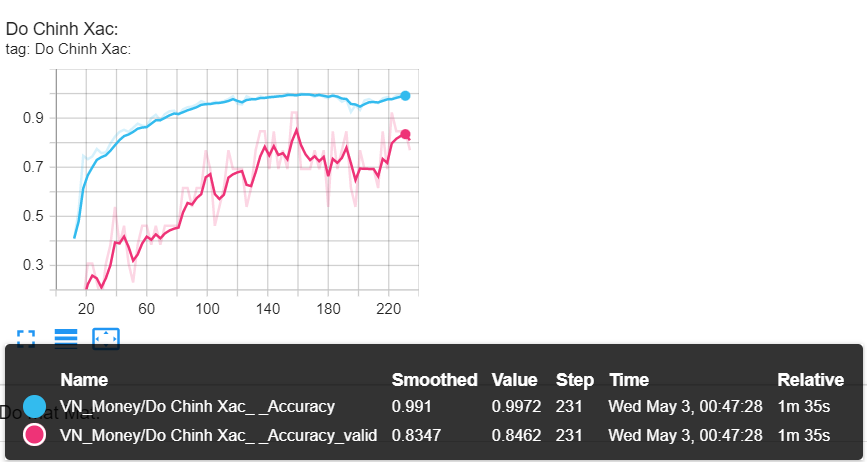
\includegraphics[scale = 0.6]{Img/Money/P2.png}
\end{figure}

\par - Dưới dây là dồ thị của độ mất mát. Màu xanh của tập train và màu cam của tập validation. Chi tiết xem thêm tại đây [14]
\begin{figure}[h] %% [h] --> here
    \centering
    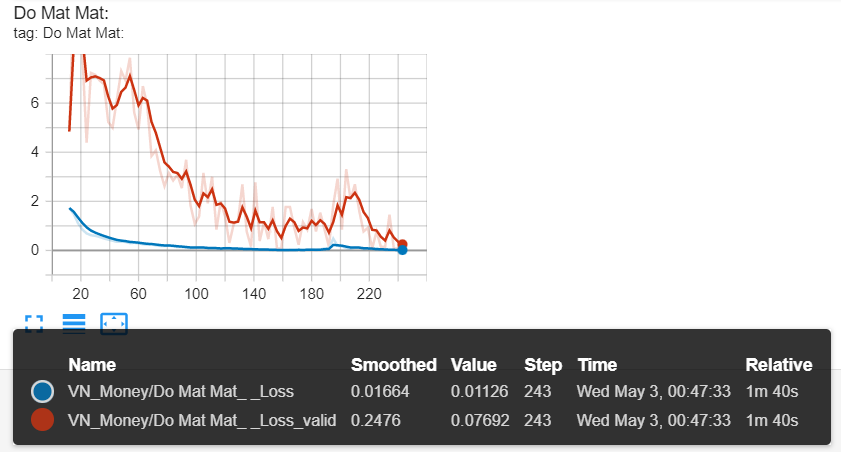
\includegraphics[scale = 0.65]{Img/Money/P3.png}
\end{figure}
\par - Tiến hành lưu và load model 

\begin{python}
In [8]: # Save model
        FILE = "model.pth"
        torch.save(model.state_dict(), FILE)
        
        
        # Load model
        loaded_model = CNN().to(device)
        loaded_model.load_state_dict(torch.load(FILE)) # it takes the loaded dictionary, not the path file itself
        loaded_model.eval()
\end{python}
\newpage
\begin{minted}{bash}
Out [8]:
    CNN(
      (maxpool): MaxPool2d(kernel_size=2, stride=2, padding=0, dilation=1, 
                            ceil_mode=False)
      (conv1): Conv2d(3, 32, kernel_size=(3, 3), stride=(1, 1), padding=(2, 2))
      (conv2): Conv2d(32, 64, kernel_size=(3, 3), stride=(1, 1), padding=(1, 1))
      (conv3): Conv2d(64, 128, kernel_size=(3, 3), stride=(1, 1), padding=(1, 1))
      (avgpool): AdaptiveAvgPool2d(output_size=(7, 7))
      (dropout): Dropout(p=0.1, inplace=False)
      (fc1): Linear(in_features=6272, out_features=124, bias=True)
      (fc2): Linear(in_features=124, out_features=32, bias=True)
      (fc3): Linear(in_features=32, out_features=6, bias=True)
    )
\end{minted}
\par - Cuối cùng ta tiến hành thử nghiệm model với ảnh từ tập test.
\begin{python}
In [9]: from torchvision import transforms
        import PIL.Image as Image 
        url = '/kaggle/input/vn-money/Money/Test/500k.jpg'
        # Load anh
        img = Image.open(url)
        # Hien thi anh
        plt.imshow(img)
        plt.show()
        # Ap dung transform
        img_transformed = transform(img)
        test = loaded_model(img_transformed.to(device))
        print(class_name[torch.max(test.data,1)[1].data])
\end{python}


\begin{figure}[h] %% [h] --> here
    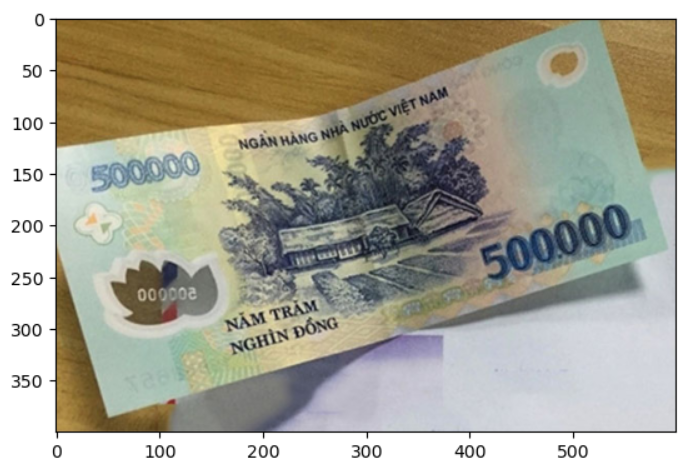
\includegraphics[scale = 0.8]{Img/Money/P4.png}
\end{figure}
\begin{minted}{bash}
Out [10]: 500k
\end{minted}



\newpage
\subsection{Recognition of all members of class from face images (you collected)}
\par \textbf{Code đầy đủ ở đây [10]}
\par\hspace{0cm}- Đầu tiên ta sẽ import các thư viện cần thiết cho việc xây dựng và thực thi model
\par\hspace{0cm}- Ở đây ta sẽ dùng Cuda cho việc xây model trên GPU và nó giúp ta tăng tống quá trình train và thực thi model

\begin{python}
In [1]: import numpy as np
        from tqdm import tqdm
        import torch
        import torch.nn as nn
        import torchvision
        import torch.nn.functional as F
        from torch.utils.data import DataLoader
        from torchvision import datasets, transforms, models
        from torchvision.transforms import ToTensor
        import matplotlib.pyplot as plt
        from torch.utils.tensorboard import SummaryWriter
        
        
        device = torch.device('cuda' if torch.cuda.is_available() else 'cpu')
        print(device)
\end{python}

\begin{minted}{bash}
Out [1]: cuda
\end{minted}
\par - Tiếp Theo ta sẽ xây dựng hàm transform để biến đổi trên dữ liệu (data augmentation) hoặc chuẩn hóa (data normalization) dữ liệu trước khi đưa vào huấn luyện mô hình.
\par - Việc sử dụng hàm transform giúp cho mô hình huấn luyện được đào tạo trên nhiều dữ liệu
đa dạng hơn, giúp mô hình học được các đặc trưng tổng quát hơn và tránh overfitting trên dữ liệu huấn luyện.
\par - Quy trình của hàm transform: Thay đổi kích thước ảnh về dạng (32x32) $\Rightarrow$ Chuyển về dạng tensor $\Rightarrow$ Chuẩn hóa ma trận.

\begin{python}
In [2]: transform = transforms.Compose([
                transforms.RandomRotation(10),      
                transforms.RandomHorizontalFlip(),  
                transforms.Resize(32),             
                transforms.CenterCrop(32),         
                transforms.ToTensor(),
                transforms.Normalize([0.485, 0.456, 0.406],
                                     [0.229, 0.224, 0.225])
        ])
        
        class FaceDataset(torch.utils.data.Dataset):
            def __init__(self, root, transform = None):
                self.data = datasets.ImageFolder(root, transform = transform)
                self.classes = self.data.classes
                self.num_classes = len(self.classes)
            def __getitem__(self, index):
                img, label = self.data[index]
                one_hot_label = F.one_hot(torch.tensor(label), num_classes=self.num_classes).float()
                return img, one_hot_label   
            
            def __len__(self):
                    return len(self.data)
                
                
        x_train = FaceDataset( root=("/kaggle/input/face-class/Face/Train"), transform = transform)
        x_val = FaceDataset(root = ('/kaggle/input/face-class/Face/Val'), transform = transform)
\end{python}

\par - Tiếp theo ta sẽ tiến hành thiết lập siêu tham số (hyperparameter) và chia dữ liệu theo batch
cho model
\par - Ở đây ta sử dụng Weight Decay (L2 Regularization) bằng 0.0001 để giảm thiểu Overfitting [5]
\begin{python}
In [3]: print("Tong class: ",len(x_train.classes))
        print("Ten cac loai: ",x_train.classes)
        class_name = ['Cao Minh Quan', 'Huynh Anh Duy', 'Le Tri Dung', 'Nguyen Hai Hoang', 'Nguyen Ngoc Nhan']
        
        batch = 128
        epochs = 12
        learning_rate = 1e-3
        weight_decay = 1e-4
        
        train_loader = DataLoader(x_train, batch_size = batch, shuffle = True)
        val_loader = DataLoader(x_val, batch_size = batch, shuffle = True)
        
        examples = iter(val_loader)
        example_data, example_targets = next(examples)
\end{python}

\begin{minted}{bash}
Out [3]: Tong class:  5
         Ten cac loai:  ['CaoMinhQuan', 'HuynhAnhDUy', 'LeTriDung', 'NguyenHaiHoang', 'NguyenNgocNhan']

\end{minted}


\newpage
\par - Tiếp theo ta sẽ tiến hành xây dựng model CNN
\par - Dưới đây là hình ảnh cấu trúc model CNN. Chi tiết xem thêm tại đây[15]

\begin{figure}[h] %% [h] --> here
    \centering
    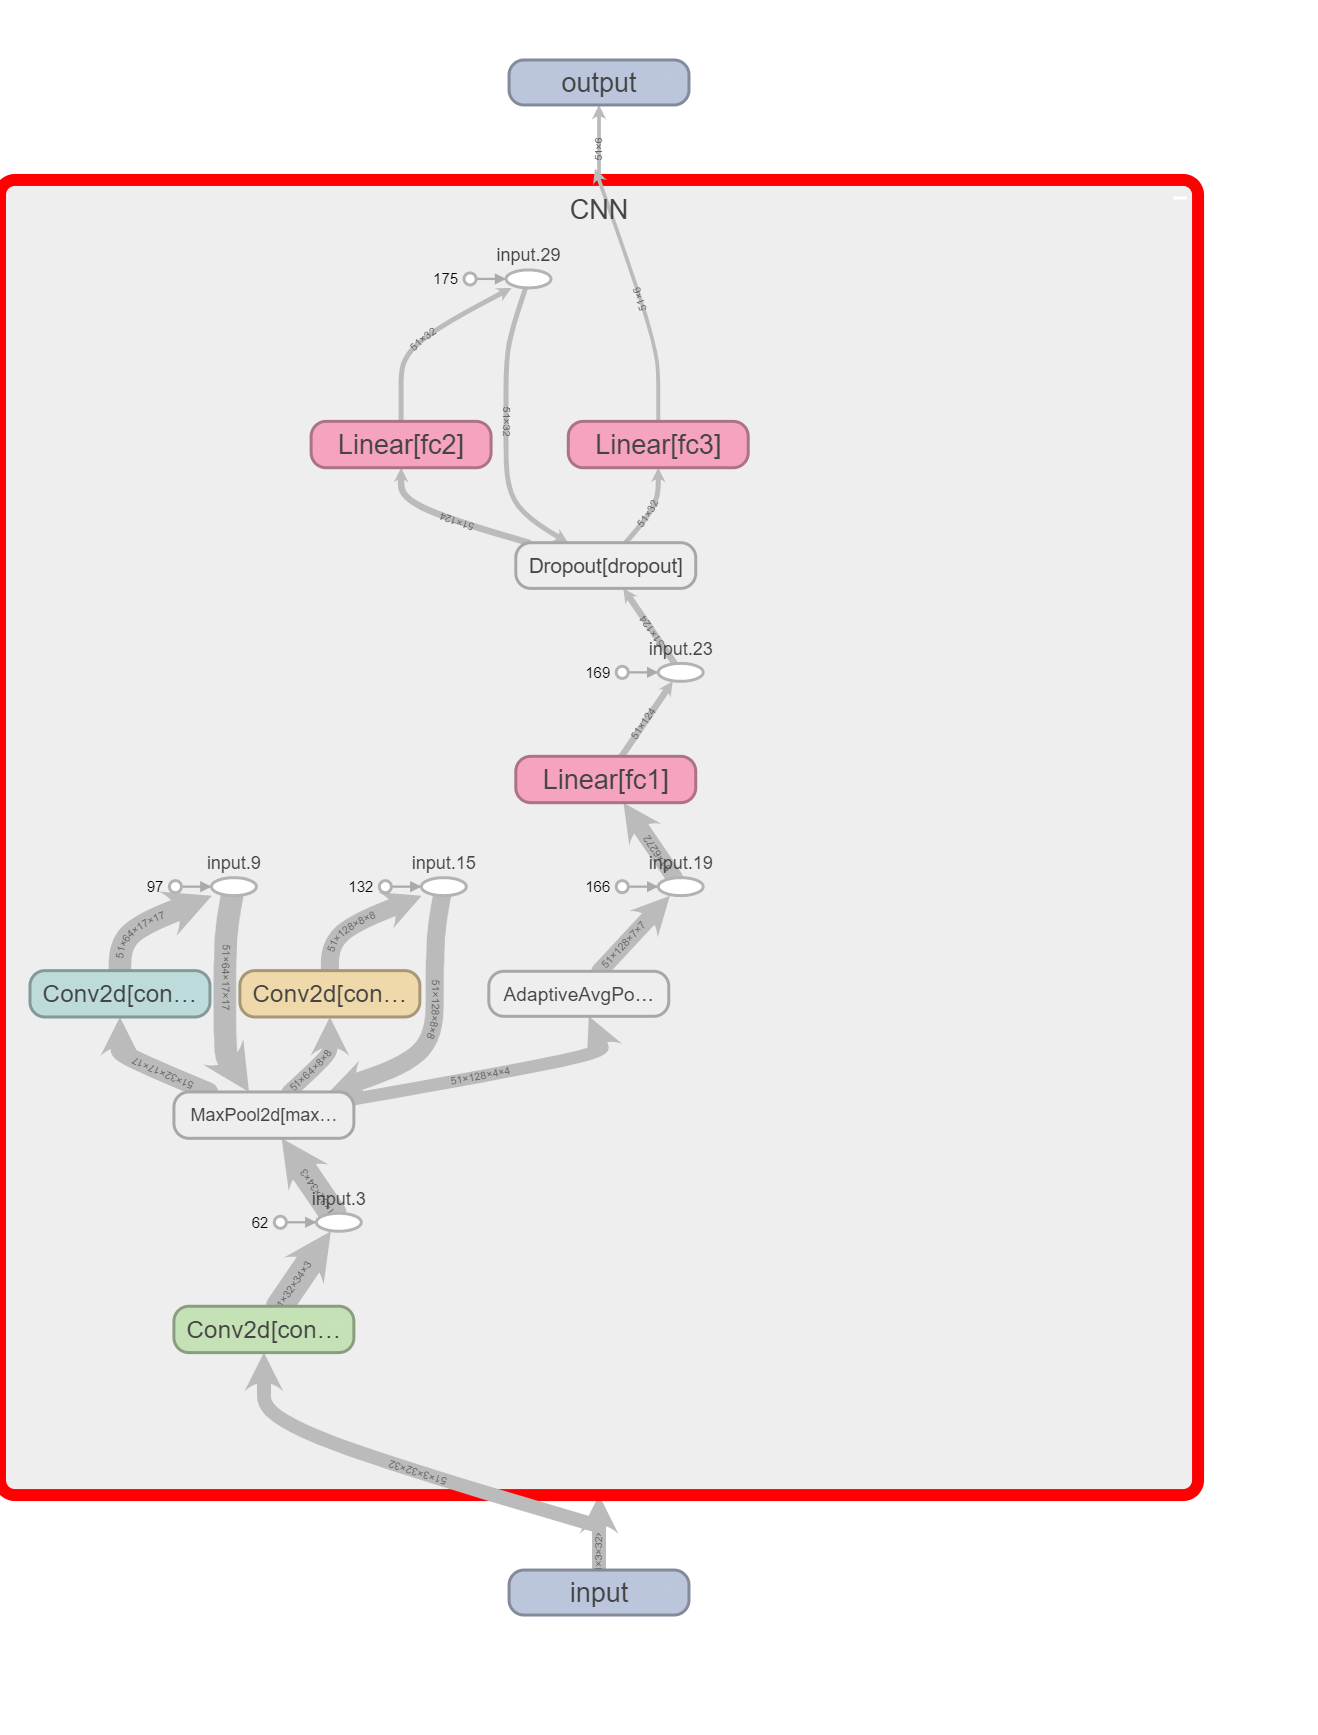
\includegraphics[scale = 0.2]{Img/Face/P1.png}
\end{figure}
\begin{python}
In [4]: class CNN(nn.Module):
          def __init__(self):
            super(CNN, self).__init__()
            self.maxpool = nn.MaxPool2d(kernel_size = 2, stride = 2)
            self.conv1 = nn.Conv2d(3,32,3,stride = 1, padding = 2)
            self.conv2 = nn.Conv2d(32,64,3,stride = 1, padding = 1)
            self.conv3 = nn.Conv2d(64,128,3,stride = 1, padding = 1)
            self.avgpool = nn.AdaptiveAvgPool2d((7, 7))
            self.dropout = nn.Dropout(p = 0.1)
            self.fc1 = nn.Linear(7*7*128, 124)
            self.fc2 = nn.Linear(124,32)
            self.fc3 = nn.Linear(32, 6)
          def forward(self, x):
            x = self.maxpool(F.leaky_relu(self.conv1(x)))
            x = self.maxpool(F.leaky_relu(self.conv2(x)))
            x = self.maxpool(F.leaky_relu(self.conv3(x)))
            x = self.avgpool(x)
            x = x.view(-1, 7*7*128)
            x = self.dropout(F.leaky_relu(self.fc1(x)))
            x = self.dropout(F.leaky_relu(self.fc2(x)))
            x = self.fc3(x)
            return x
        model = CNN().to(device)
        criterion = nn.CrossEntropyLoss()
        optimizer = torch.optim.Adam(model.parameters(), lr = learning_rate, weight_decay = weight_decay)
\end{python}
\newpage
\begin{python}
In [5]: from prettytable import PrettyTable
        
        def count_parameters(model):
            table = PrettyTable(["Modules", "Parameters"])
            total_params = 0
            for name, parameter in model.named_parameters():
                if not parameter.requires_grad: 
                    continue
                param = parameter.numel()
                table.add_row([name, param])
                total_params+=param
            print(table)
            print(f"Total Trainable Params: {total_params}")
            return total_params
        
        count_parameters(model)
\end{python}


\begin{minted}{bash}
    +--------------+------------+
    |   Modules    | Parameters |
    +--------------+------------+
    | conv1.weight |    864     |
    |  conv1.bias  |     32     |
    | conv2.weight |   18432    |
    |  conv2.bias  |     64     |
    | conv3.weight |   73728    |
    |  conv3.bias  |    128     |
    |  fc1.weight  |   777728   |
    |   fc1.bias   |    124     |
    |  fc2.weight  |    3968    |
    |   fc2.bias   |     32     |
    |  fc3.weight  |    192     |
    |   fc3.bias   |     6      |
    +--------------+------------+
    Total Trainable Params: 875298
Out [5]: 875298
\end{minted}
\par - Tổng có 875298 tham số
\vspace{0.5cm}
\par - Tiếp theo ta sẽ tiến hành train và đánh giá model
\newpage
\begin{python}
In [6]:
n_total_steps = len(train_loader)

run_loss = 0.0
run_acc = 0.0
for epoch in range(epochs):
    for i, (images, labels) in enumerate(tqdm(train_loader)):
        images = images.reshape(-1,3,32,32).to(device)
        labels = labels.to(device)
        _, labels = torch.max(labels.data, 1)

        outputs = model(images)

        loss = criterion(outputs,labels)
        
        run_loss +=loss.item() #for tensorboard
        _,pred = torch.max(outputs.data, 1)
        run_acc += (pred==labels).sum().item()#for tensorboard
        
        optimizer.zero_grad()
        loss.backward()
        optimizer.step()
        
        if (i+1) % 2 == 0:     
            with torch.no_grad():
                n_correct = 0
                n_samples = 0
                n_class_correct = [0 for i in range(5)]
                n_class_samples = [0 for i in range(5)]
                
                for images_val, labels_val in val_loader:
                    images_val = images_val.reshape(-1,3,32,32).to(device)
                    labels_val = labels_val.to(device)
                    _, labels_val = torch.max(labels_val.data, 1)
                    
                    output_val = model(images_val)
                    _, predict_val = torch.max(output_val.data, 1)
                    n_samples += labels_val.size(0)
                    n_correct += (predict_val == labels_val).sum().item()
                    loss_val = F.mse_loss(labels_val.float(),predict_val.float())
                    for i in range(26):
                        label_val = labels_val[i]
                        pred_val = predict_val[i]
                        if label_val == pred_val:
                            n_class_correct[label_val] += 1
                            
                        n_class_samples[label_val] += 1      
                acc_val = n_correct/(n_samples)
                acc_total = run_acc/((2-1)*128+pred.size(0))
                print(f'Epoch[{epoch+1}/{epochs}]:  Loss_Train: {(run_loss/2):.2f}, Acc_Train: {acc_total:.2f}, Loss_Val: {loss_val:.2f}, Acc_Val: {acc_val:.2f}')

print('Finished Training')
\end{python}


\begin{minted}{bash}
100%[==========] 2/2 [00:22<00:00, 11.44s/it]
Epoch[1/12]:  Loss_Train: 1.74, Acc_Train: 0.18, Loss_Val: 4.47, Acc_Val: 0.16
100%[==========] 2/2 [00:17<00:00,  8.71s/it]
Epoch[2/12]:  Loss_Train: 1.54, Acc_Train: 0.29, Loss_Val: 3.37, Acc_Val: 0.33
100%[==========] 2/2 [00:17<00:00,  8.67s/it]
Epoch[3/12]:  Loss_Train: 1.34, Acc_Train: 0.39, Loss_Val: 2.08, Acc_Val: 0.51
100%[==========] 2/2 [00:16<00:00,  8.37s/it]
Epoch[4/12]:  Loss_Train: 1.05, Acc_Train: 0.62, Loss_Val: 1.67, Acc_Val: 0.63
100%[==========] 2/2 [00:17<00:00,  8.90s/it]
Epoch[5/12]:  Loss_Train: 0.78, Acc_Train: 0.79, Loss_Val: 0.37, Acc_Val: 0.75
100%[==========] 2/2 [00:17<00:00,  8.57s/it]
Epoch[6/12]:  Loss_Train: 0.51, Acc_Train: 0.82, Loss_Val: 0.27, Acc_Val: 0.84
100%[==========] 2/2 [00:17<00:00,  8.90s/it]
Epoch[7/12]:  Loss_Train: 0.40, Acc_Train: 0.87, Loss_Val: 0.49, Acc_Val: 0.78
100%[==========] 2/2 [00:17<00:00,  8.88s/it]
Epoch[8/12]:  Loss_Train: 0.34, Acc_Train: 0.88, Loss_Val: 0.22, Acc_Val: 0.84
100%[==========] 2/2 [00:17<00:00,  8.54s/it]
Epoch[9/12]:  Loss_Train: 0.24, Acc_Train: 0.89, Loss_Val: 0.18, Acc_Val: 0.82
100%[==========] 2/2 [00:17<00:00,  8.84s/it]
Epoch[10/12]:  Loss_Train: 0.12, Acc_Train: 0.93, Loss_Val: 0.12, Acc_Val: 0.88
100%[==========] 2/2 [00:17<00:00,  8.64s/it]
Epoch[11/12]:  Loss_Train: 0.11, Acc_Train: 0.95, Loss_Val: 0.25, Acc_Val: 0.90
100%[==========] 2/2 [00:17<00:00,  8.79s/it]
Epoch[12/12]:  Loss_Train: 0.08, Acc_Train: 0.96, Loss_Val: 0.08, Acc_Val: 0.92
Finished Training
    
\end{minted}

\begin{python}
In [7]: with torch.no_grad():
            n_correct = 0
            n_samples = 0
            n_class_correct = [0 for i in range(5)]
            n_class_samples = [0 for i in range(5)]
            for images, labels in val_loader:
                images = images.reshape(-1,3,32,32).to(device)
                labels = labels.to(device)
                _, labels = torch.max(labels.data, 1)
                output = model(images)
                _, predict = torch.max(output.data, 1)
                n_samples += labels.size(0)
                n_correct += (predict == labels).sum().item()
                for i in range(51):
                    label = labels[i]
                    pred = predict[i]
                    if label == pred:
                        n_class_correct[label] +=1
                    n_class_samples[label]+=1     
            acc = 100.0*n_correct/n_samples
            print(f'Accuracy of the network: {acc} %')
\end{python}
\begin{minted}{bash}
Out [8]: Accuracy of the network: 92.15686274509804 %
\end{minted}

\par- Sau 12 epochs ta có thể thấy độ chính xác trên tập validation là 92 $\%$
\par- Dưới dây là dồ thị của độ chính xác. Màu xanh của tập train và màu hồng của tập validation.
Chi tiết xem thêm tại đây [15]

\begin{figure}[h] %% [h] --> here
    \centering
    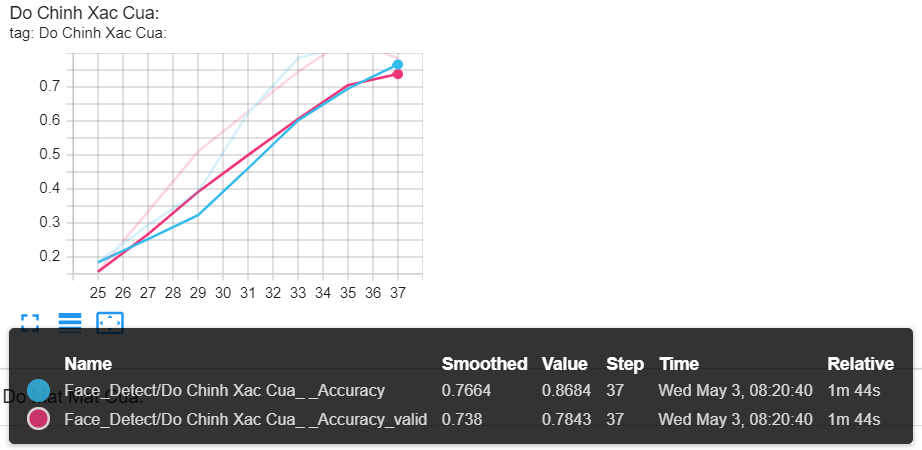
\includegraphics[scale = 0.6]{Img/Face/P2.png}
\end{figure}

\par - Dưới dây là dồ thị của độ mất mát. Màu xanh của tập train và màu cam của tập validation. Chi tiết xem thêm tại đây [15]
\begin{figure}[h] %% [h] --> here
    \centering
    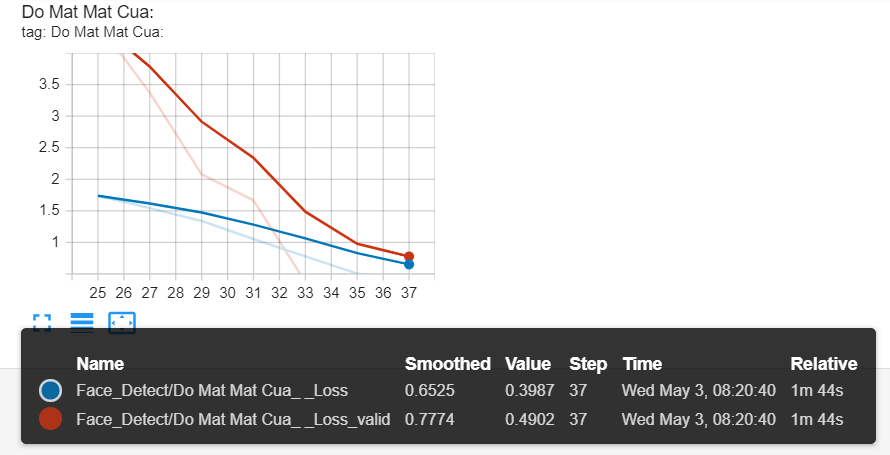
\includegraphics[scale = 0.65]{Img/Face/P3.png}
\end{figure}
\par - Tiến hành lưu và load model 
\begin{python}
In [9]: # Save model
        FILE = "model_face.pth"
        torch.save(model.state_dict(), FILE)
        
        # Load model
        loaded_model = CNN().to(device)
        loaded_model.load_state_dict(torch.load(FILE)) # it takes the loaded dictionary, not the path file itself
        loaded_model.eval()
\end{python}
\newpage
\begin{minted}{bash}
Out [9]:
    CNN(
      (maxpool): MaxPool2d(kernel_size=2, stride=2, padding=0, dilation=1, 
                            ceil_mode=False)
      (conv1): Conv2d(3, 32, kernel_size=(3, 3), stride=(1, 1), padding=(2, 2))
      (conv2): Conv2d(32, 64, kernel_size=(3, 3), stride=(1, 1), padding=(1, 1))
      (conv3): Conv2d(64, 128, kernel_size=(3, 3), stride=(1, 1), padding=(1, 1))
      (avgpool): AdaptiveAvgPool2d(output_size=(7, 7))
      (dropout): Dropout(p=0.1, inplace=False)
      (fc1): Linear(in_features=6272, out_features=124, bias=True)
      (fc2): Linear(in_features=124, out_features=32, bias=True)
      (fc3): Linear(in_features=32, out_features=6, bias=True)
    )
\end{minted}


\par - Cuối cùng ta tiến hành thử nghiệm model với ảnh từ tập test.
\begin{python}
In [10]:from torchvision import transforms
        import PIL.Image as Image
        url = '/kaggle/input/face-class/Face/Test/NguyenNgocNhan.jpg'
        # Load anh
        img = Image.open(url)
        # Hien thi anh
        plt.imshow(img)
        plt.show()
        # Ap dung transform
        img_transformed = transform(img)   
        # App load model
        test = loaded_model(img_transformed.to(device))
        print(class_name[torch.max(test.data,1)[1].data])
\end{python}
\begin{figure}[h] %% [h] --> here
    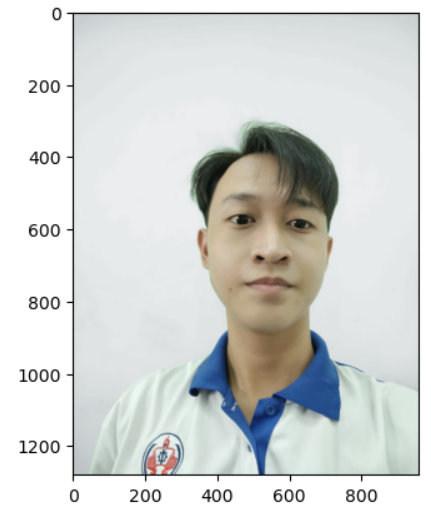
\includegraphics[scale = 0.8]{Img/Face/P4.png}
\end{figure}

\begin{minted}{bash}
Out[10]:Nguyen Ngoc Nhan
\end{minted}





%-------------------------------------------------------------
\newpage
\section{Results - Kết quả}
\par -  Sau khi sử dụng CNN với độ chính xác trên 80$\%$ là một thành công hơn so với các mô hình machine learning trong việc xử lý ảnh và phân loại các đối tượng. Nó phụ thuộc rất nhiều vào các siêu tham số (hyperparameters) như epochs, batch size, dropout, weight decay, optimizer. 
\par - Với CNN, chúng ta có thể tạo ra các mô hình phân loại ảnh chất lượng cao và đáng tin cậy, đặc biệt là trong các bài toán phân loại ảnh có tính chất phức tạp như phân loại hoa, phân loại động vật, nhận diện khuôn mặt, và nhiều bài toán khác. CNN đã trở thành một công cụ quan trọng trong lĩnh vực xử lý ảnh và thường được sử dụng để giải quyết các bài toán phân loại ảnh trong các ứng dụng thực tế.
%-------------------------------------------------------------
\section{Conclusions - Kết luận}
\par - Convolutional neural network (CNN) là một loại mạng nơ-ron nhân tạo rất phổ biến trong việc xử lý ảnh và nhận dạng hình ảnh. Nó được thiết kế để phát hiện các đặc trưng của ảnh thông qua các lớp tích chập và kết hợp chúng lại để tạo ra một dự đoán cuối cùng.
\par - CNN đã đạt được những thành tựu lớn trong lĩnh vực nhận dạng hình ảnh, bao gồm nhận dạng khuôn mặt, phân loại hình ảnh, nhận dạng vật thể và nhiều ứng dụng khác. Nó cũng được sử dụng trong nhiều lĩnh vực khác nhau bao gồm xử lý ngôn ngữ tự nhiên, nhận dạng giọng nói, xử lý tín hiệu và nhiều ứng dụng khác.
\par - Mặc dù CNN đã đạt được nhiều thành tựu đáng kể, nhưng vẫn còn nhiều thách thức cần giải quyết, bao gồm độ chính xác của mô hình, kích thước mô hình và thời gian huấn luyện. Tuy nhiên các pretrain model hiện nay thường được xây dựa trên mạng CNN và các biến thể của nó. 















%-------------------------------------------------------------

\newpage
\section{References}
\par \hspace{1cm} [1] https://medium.com/@RaghavPrabhu/understanding-of-convolutional-neural-network-cnn-deep-learning-99760835f148
\par \hspace{1cm} [2] https://nttuan8.com/bai-6-convolutional-neural-network/
\par \hspace{1cm} [3] https://viblo.asia/p/deep-learning-tim-hieu-ve-mang-tich-chap-cnn-maGK73bOKj2
\par \hspace{1cm} [4] https://aicurious.io/blog/2019-09-23-cac-ham-kich-hoat-activation-function-trong-neural-networks
\par \hspace{1cm} [5] https://machinelearningcoban.com/2017/03/04/overfitting/
\vspace{0.5cm}
\par \textbf{GitHub: }https://github.com/tooniesnguyen/
\par \hspace{1cm} [6] https://github.com/tooniesnguyen/AI-UTE/blob/main/Notebooks/MidtermProject
\par \hspace{0cm}/predict-future.ipynb

\par \hspace{1cm} [7] https://github.com/tooniesnguyen/AI-UTE/blob/main/Notebooks/MidtermProject
\par /miniproject-flowers.ipynb
\par \hspace{1cm} [8] https://github.com/tooniesnguyen/AI-UTE/blob/main/Notebooks/MidtermProject
\par /vn-dishes.ipynb
\par \hspace{1cm} [9] https://github.com/tooniesnguyen/AI-UTE/blob/main/Notebooks/MidtermProject
\par /predict-money.ipynb
\par \hspace{1cm} [10] https://github.com/tooniesnguyen/AI-UTE/blob/main/Notebooks/MidtermProject
\par /face-detect.ipynb
\vspace{0.5cm}

\par \textbf{TensorBoard: }https://huggingface.co/Toonies/
\par \hspace{1cm} [11] https://huggingface.co/Toonies/PredictFuture/tensorboard
\par \hspace{1cm} [12] https://huggingface.co/Toonies/Flowers/tensorboard
\par \hspace{1cm} [13] https://huggingface.co/Toonies/TenDishes/tensorboard
\par \hspace{1cm} [14] https://huggingface.co/Toonies/Money/tensorboard
\par \hspace{1cm} [15] https://huggingface.co/Toonies/FaceDetect/tensorboard


\end{document}